\chapter{Architectural Design} \label{architecture}

The following section describes the architecture of the eMSP and the CPMS systems. The descriptions start from a high-level point of view, detailing interactions between all systems at play. We will focus majorly on defining the roles of the systems, to obtain a clear representation of the communication between all participants. After this description, the focus will be on the components needed to obtain the functionalities of the applications and then their deployment and runtime utilization. This section also includes a precise definition of the architectural patterns utilized to deploy all identified components and other design decisions taken in the architectural design process.

\section{Overview}

\subsection{General context}

Generally speaking, two main systems are the focus of this project, which are the eMSP and the CPMS. These two interact with each other and also with other actors:
\begin{itemize}
    \item The \textit{DSO} is used by the CPMS for querying pieces of information regarding, usually, the price of energy.
    \item The \textit{eRoaming} is used by the eMSPs for discovering all the available CPOs (with their respective CPMSs) that subscribed to the service.
    \item The \textit{PaymentService} represents a generic payment service used by both systems (the CPMS also uses it for paying the DSOs for the energy).
    \item The \textit{users} interact with their respective system.
\end{itemize}

\begin{figure}[h!]
    \centering
    \includegraphics[width=0.97\columnwidth]{./images/overview/general}
    \caption{general overview of the systems.}
\end{figure}

\subsection{eMSP composition diagram}

The following diagram presents a more precise description of the eMSP system, in which the most important components of the infrastructure are depicted. These are divided into different groups following the three-tier architecture design pattern, grouping them according to their main purpose. Moreover, the connections of the various components with external entities are pointed out. Please, note that the internal connections between components are not presented here.

\begin{figure}[h!]
    \centering
    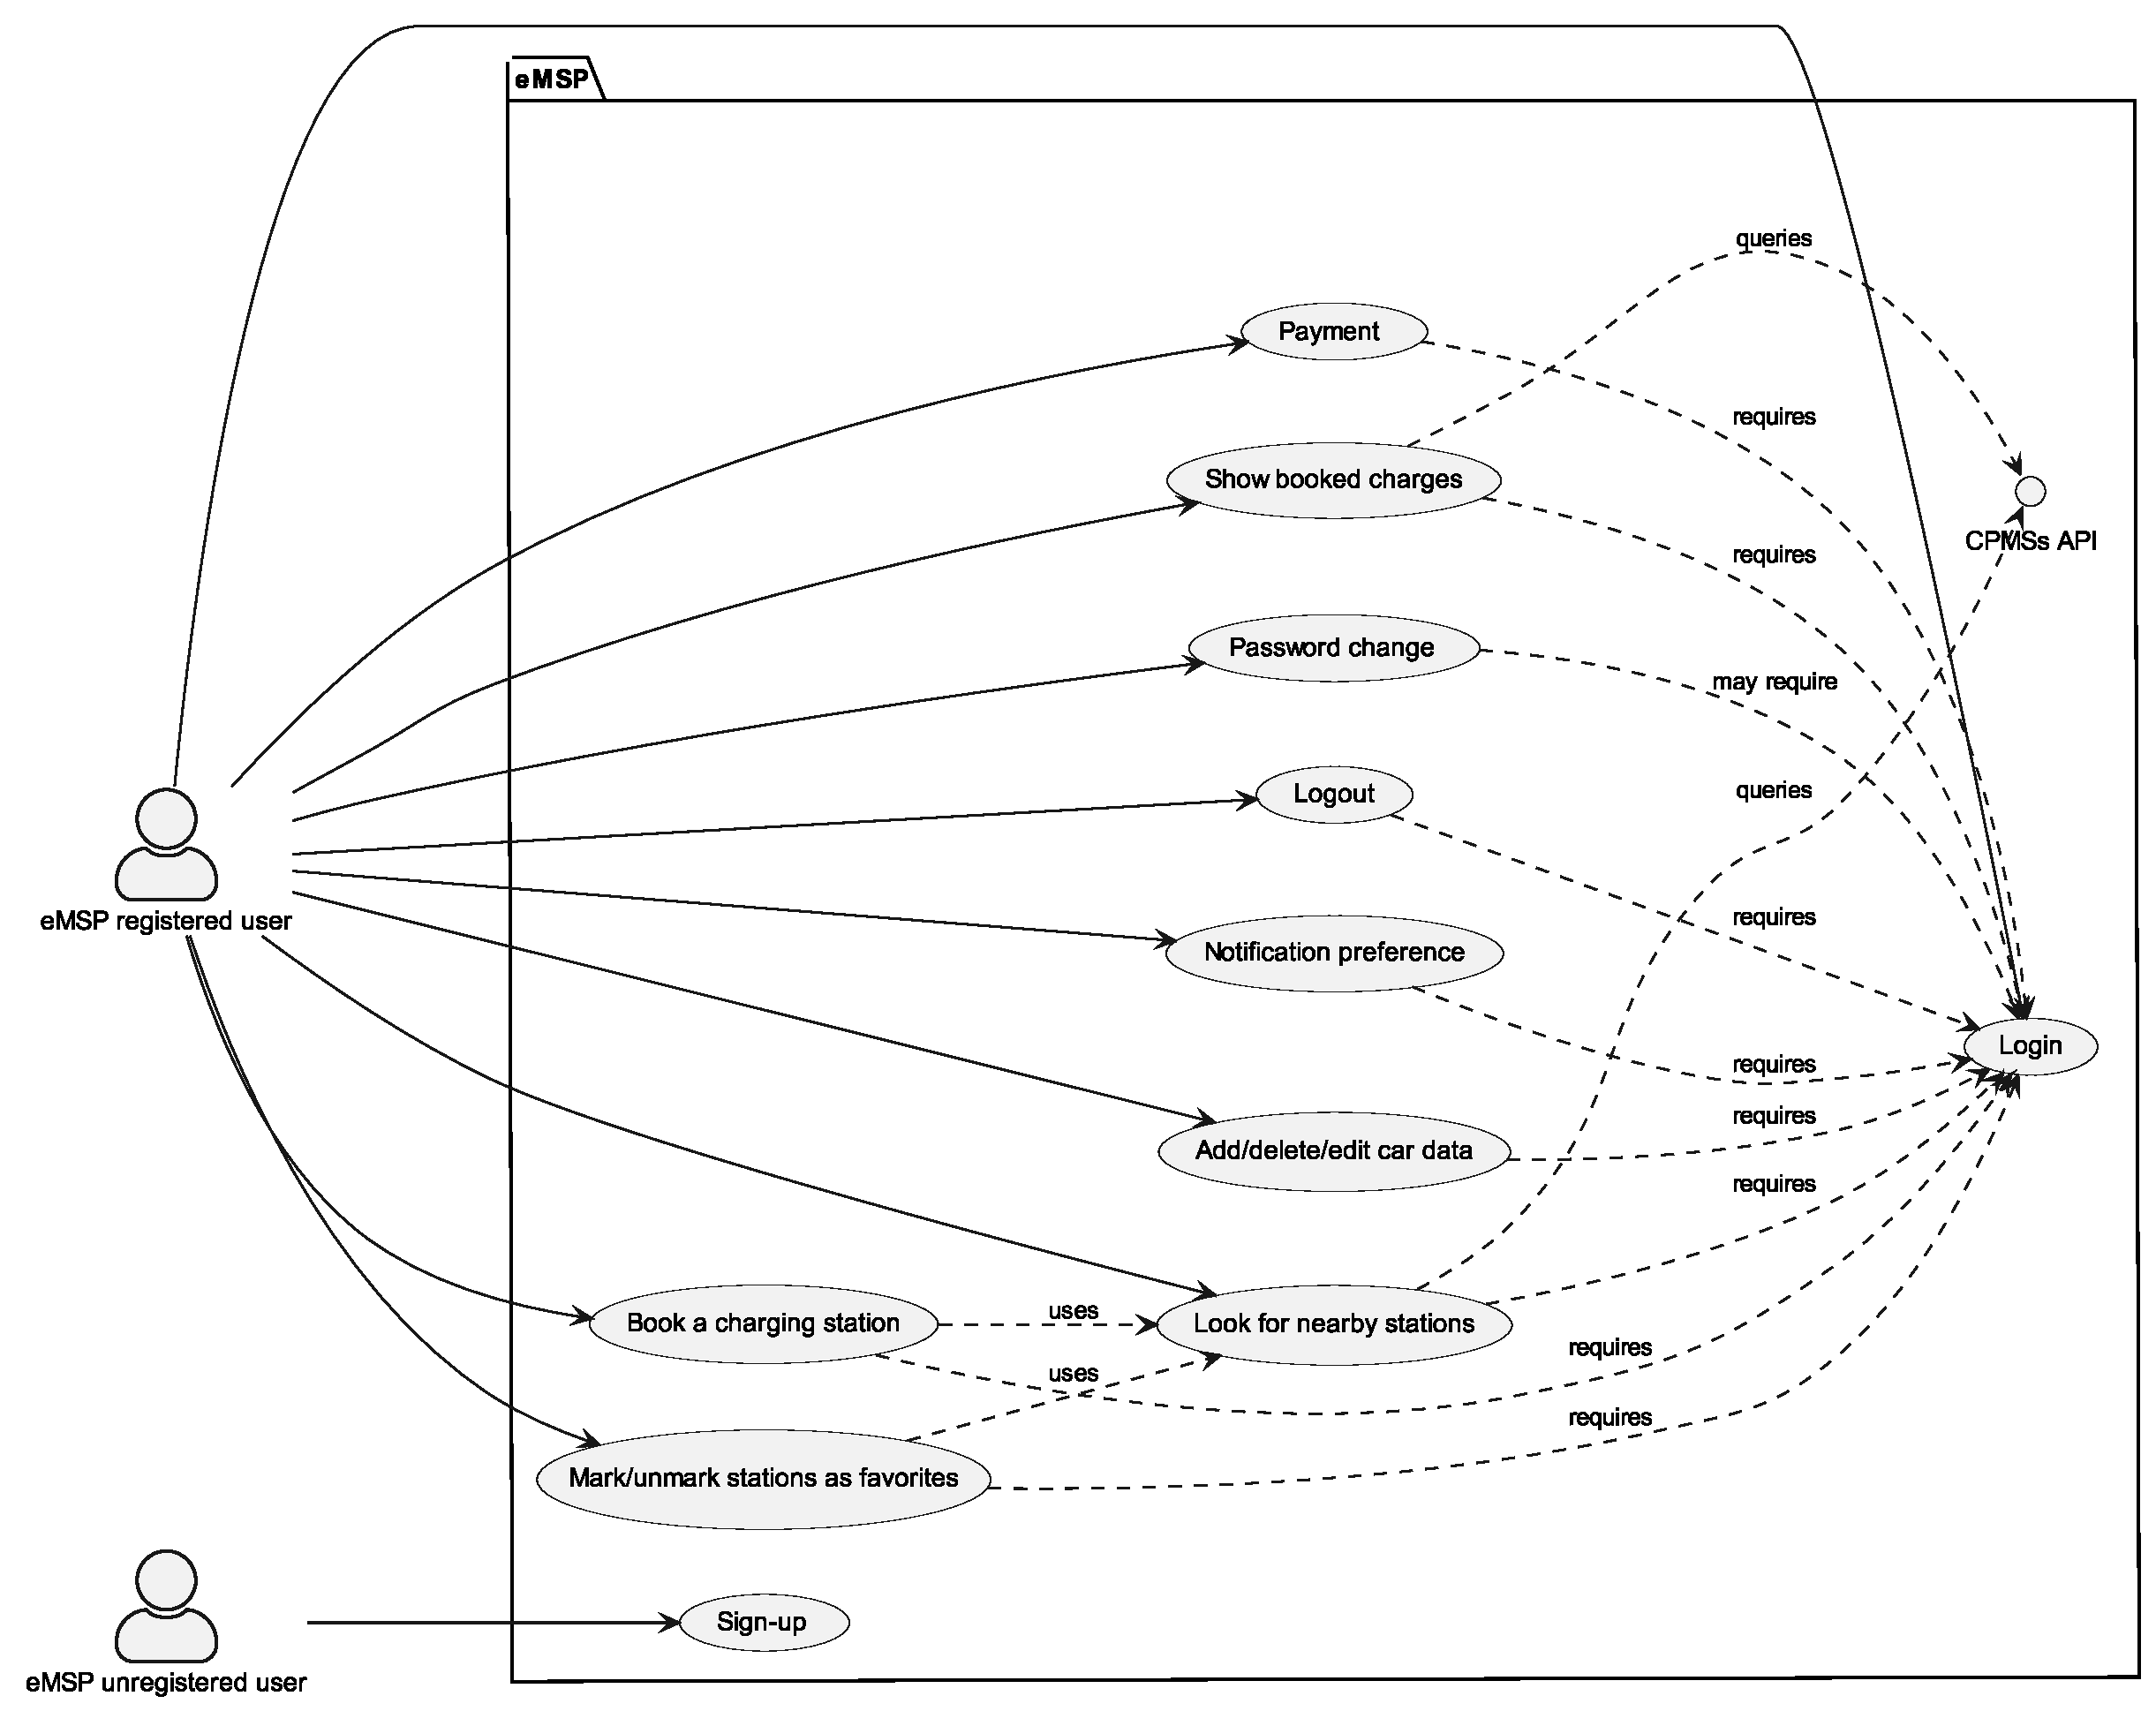
\includegraphics[width=0.79\columnwidth]{./images/overview/emsp}
    \caption{general overview of the eMSP.}
\end{figure}

\paragraph{Presentation tier} This tier is the frontend of the system, it's the one that the end user (consumer) uses for interacting with the system. It allows the user to book the charges, look for the stations, pay for the charge\dots

\paragraph{Business tier} This tier is in the middle between the presentation and the data tiers. It manages all the logic of the application but mainly interacts with the CPMS and the other external service providers in order to offer all the required functionalities to the consumer.

\paragraph{Data tier} This tier is the one that keeps track of all the user's data. It's in charge of storing, among the others, all the vehicles' certificates, which are some of the most sensible pieces of information in the whole system.

\paragraph{Other components} The other components that the system interacts with are the eRoaming service provider, which allows discovery of the various CPOs, the PaymentService for managing transactions, and OpenStreetMap for the map and address translation service.

\subsection{CPMS composition diagram}

A similar diagram to the previous one follows. It presents a more precise description of the CPMS system and its components, following the same three-tier architecture design. The main differences lie in the external components that the CPMS is connected to, as well as the internal main components.

\begin{figure}[h!]
    \centering
    \includegraphics[width=0.79\columnwidth]{./images/overview/cpms}
    \caption{general overview of the CPMS.}
\end{figure}

\paragraph{Presentation tier} This tier is the frontend of the system, it's the one that the authorized users use for interacting with the system. It allows visualizing data about a charging station, selecting a DSO, changing the energy mix, and creating a new special offer, as well as actions related to the ones listed. 

\paragraph{Business tier} This tier is in the middle between the presentation and the data tiers. It manages all the logic of the application but mainly interacts with external service providers to offer all the required functionalities.

\paragraph{Data tier} This tier is the one that keeps track of all data used by the system. Particular attention is paid to data provided by the station sensors, and booking information derived from eMSP users.

\paragraph{Other components} The other components that the system interacts with are the eRoaming service provider (needed to let eMSPs know about the CPMS), the payment service (to receive payments from end users and to pay the energy from DSOs), the eMSP and the DSOs.

\section{Component view}

This part focuses on the inner architecture of each system, pointing out the connections between all the inner components and the ones with any external component which has to interact with this system. Moreover, all the various interfaces are depicted in this section, even though they are better explained in section \reference{view:interfaces} and \reference{view:runtime}.\medskip

For convenience, the two views of the eMSP and the CPMS are divided, to better understand the two very different subsystems of this project, focusing on their duties.

\subsection{eMSP component view}

This component diagram shows the internal structure of the eMSP system and the connections it establishes with the other components. All the internal components are briefly described right after the diagram. Please, note that also the CPMS is treated as an external component since the description of how it internally works is written in the following subsection.

\begin{figure}[h!]
    \centering
    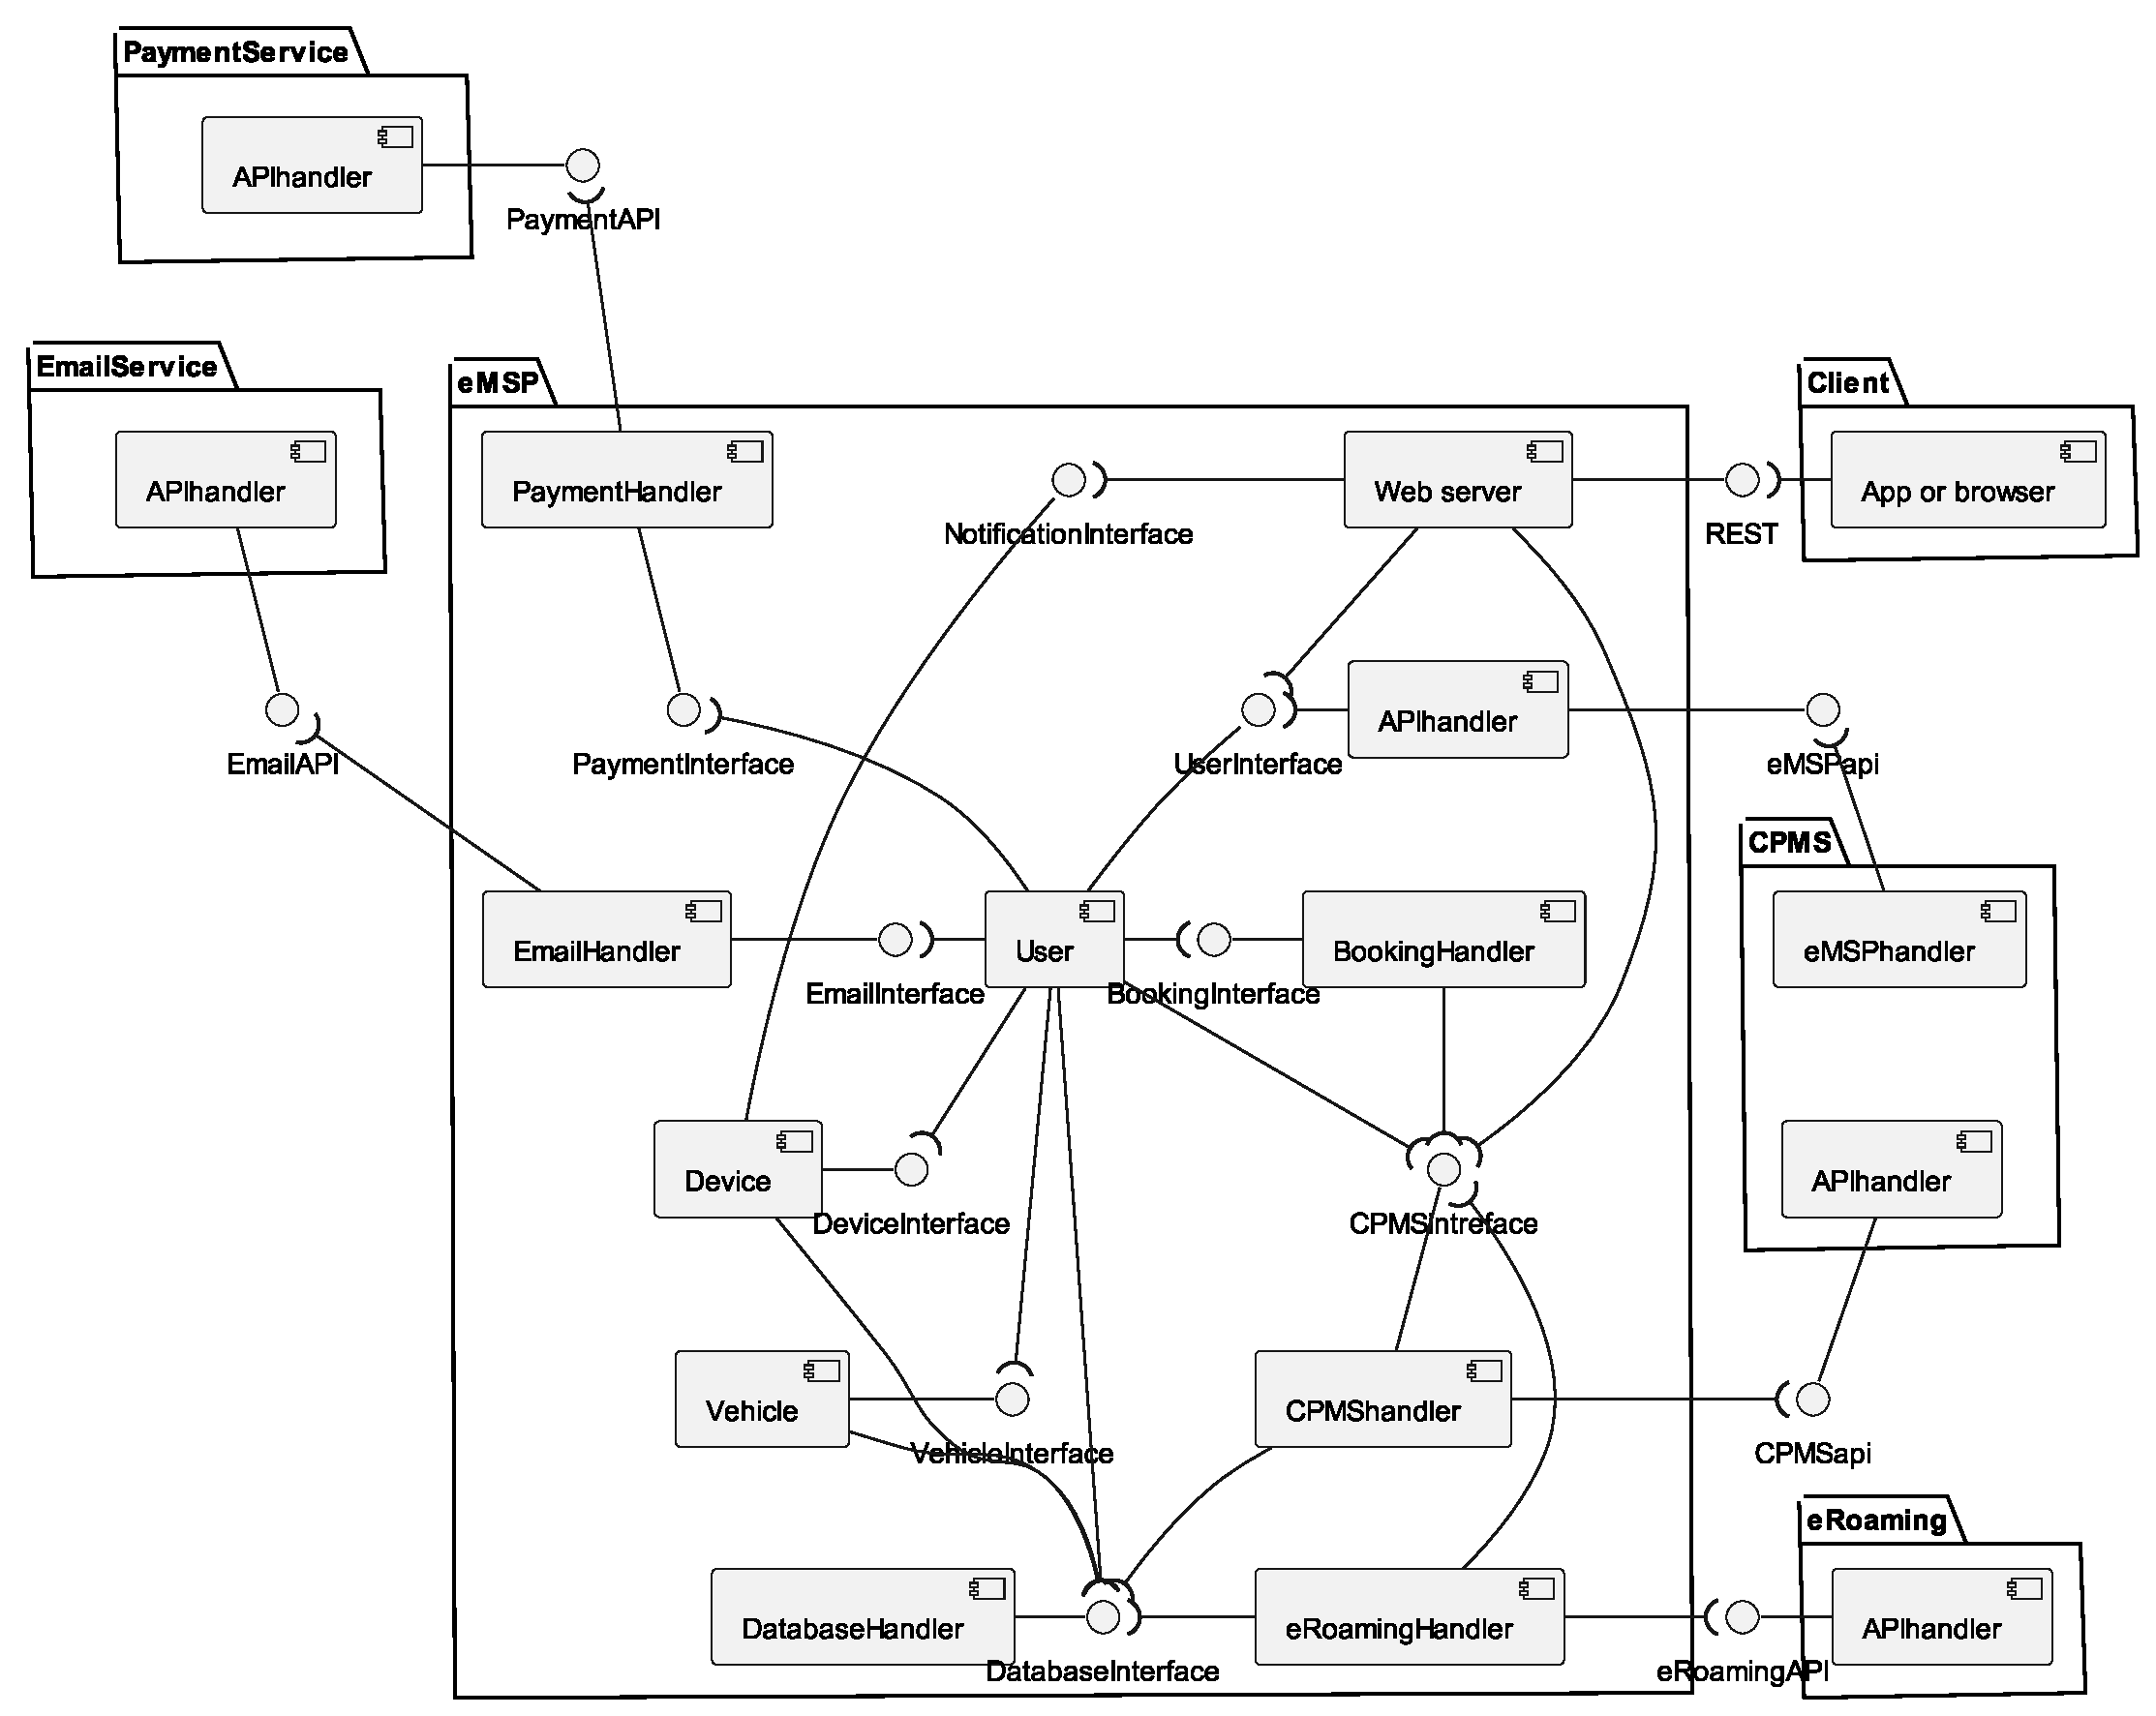
\includegraphics[width=\columnwidth]{./images/components/emsp}
    \caption{connections and interfaces of the eMSP.}
\end{figure}

\paragraph{APIhandler} Manages all the requests coming from any connected CPMS, providing the required data and sending notifications to the user whenever they're needed.

\paragraph{BookingHandler} Manages all the bookings. This is the component that, working together with the \linebreak \texttt{CPMShandler}, allows the user to book a charge, edit and delete it. Please, note that this component is not depicted in the class diagram of the \textit{Requirements Analysis and Specification Document}. This is because here, from an implementation point of view, it's better to separate these functionalities from the \texttt{User} class.

\paragraph{CPMShandler} This is the middleware between the eMPS and the CPMS. It manages all the outgoing requests for the CPMS, like the bookings and any eventual successful payment from the user.

\paragraph{DatabaseHandler} The database contains all the data of the system, and together with its DBMS, it provides all the required data to the above modules. The \texttt{DatabaseInterface} presented here is just a way to represent the various queries that may be done to the database. As a simplification, in the next sections (\reference{view:interfaces} and \reference{view:runtime}) the \texttt{DatabaseInterface} is stated to provide methods for accessing the data. Of course, this is not true in practice since all the queries are written in SQL.

\paragraph{Device} This component manages all the information regarding the users' devices. It is also the one that in case the preferred notification method of the user is the notification one, keeps an open channel with that specific device and sends notifications.

\paragraph{eRoamingHandler} Manages all the processes of connecting with an eRoaming service, inserting all the information about the found CPMSs (directly taken from the found CPOs) in the database.

\paragraph{PaymentHandler} Manages all the financial transactions between the various actors of the system.

\paragraph{User} This is the main component with which the user interacts. It is also the one that provides the devices and vehicle data to the other components.

\paragraph{Vehicle} This component manages all the information regarding the users' vehicles.

\paragraph{Web server} The web server is the frontend of the system for the end user. It statically serves all the page components (it doesn't render anything, it only sends HTML pages, with the required CSS and JavaScript) and replies to the user's HTTP requests through JSON strings.

\subsection{CPMS component view}

\begin{figure}[h!]
    \centering
    \includegraphics[width=\columnwidth]{./images/components/cpms}
    \caption{connections and interfaces of the CPMS.}
\end{figure}

\paragraph {APIhandler} Manages all the requests coming from any connected eMSP, providing the required data and allowing the eMSP users to book charges.

\paragraph {Booking} Handles all the booking of charges, creating and modifying the data stored in the database. It also decides which column to assign to users, communicating the choice by sending a message to the eMSP through the \texttt{eMSPhandler}.

\paragraph {ChargingColumn} Handles the physical charging of the devices. By communicating with the database it's able to establish whether to start or finish the charge based on the bookings present and the certificate of the connected car. Through its interface, it allows observers to be attached. This can be used to send a notification to the owner of the car when the charge ends, as the column itself cannot communicate to the eMSP's API. 

\paragraph {ChargingStation} Handles the choice of DSOs and energy mix in the charging station. If \doublequotes{automatic choice} is selected for either \doublequotes{DSO choice} or \doublequotes{EnergyMix}, it keeps looping querying useful updates, making decisions, and waiting a fixed amount of time, until the mode is deselected. It adds observers to \texttt{EnergySource} and \texttt{ChargingColumn} relative to the station, to have quicker access to important information. In particular, it needs to change the energy mix whenever a station battery reaches 100\% capacity, and it needs to send a message to the car owner whose car's charge ends.

\paragraph {DatabaseHandler} It handles all communication with the database, therefore is used by most components in the CPMS system.

\paragraph {DSOhandler} It handles all communication with the DSO's API. It, therefore, is invoked when the DSO choice changes or when new information from a DSO is queried.

\paragraph {eMSPhandler} It sends messages to the eMSP by communicating with its API.

\paragraph {Energy Source} It represents the various types of sources available in the charging station (batteries, solar panels, and DSO energy). It changes the amount of energy provided by the source. Observers can be attached for various reasons. In batteries, observers can be added to prevent charging over a given threshold or running below a given threshold. 

\paragraph {eRoamingHandler} It handles connections with the eRoaming.

\paragraph {PaymentHandler} It handles connections with the Payment Service, both receiving payments and allowing eMSP users to pay directly at the charging station.

\paragraph {User} It handles all actions that the CPMS user can do through the web interface. It's capable to interact with both \texttt{ChargingStation} and the database to carry out all actions and to query the required information. 

\paragraph {Web Server} It's the frontend of the CPMS website. After login, it holds information like the \texttt{CPMSuserID} and the session token, used in all internal interactions. It communicates with the user via HTTP requests and responses, sending HTML, CSS, and JavaScript files to create the views, then sending JSON strings to send the data.

\pagebreak

\section{Deployment view}

This is the deployment view of the two systems, pointing out the internal architecture of both systems, and the interconnections between themselves and with other external systems (such as the various DSOs and the eRoaming provider).

\begin{figure}[h!]
    \centering
    \includegraphics[width=0.93\columnwidth]{./images/deployment}
    \caption{deployment view of the systems.}
\end{figure}

\paragraph{Client} Depending on the system, the client can connect to it through a desktop/personal computer or through a mobile device (this one is available only for the eMSP consumer since there exists only for it a mobile application and the website is optimized for being viewed from a mobile device). From them, the clients can interact with the system, being able to do all the actions depicted in the \textit{Requirements Analysis and Specification Document}.

\paragraph{Presentation layer} The presentation layer consists of a web server, which acts as a reverse proxy for all the services behind it. In this case, the choice of using NGINX was made because of its event-based nature, and its low memory and CPU footprint. Moreover, it provides a simple configuration for load balancing of the behind components, acting as a reverse proxy (which hides these components from the outside), provides efficient data compression and encryption, which directly provides a higher ranking position in search engines (SEO), and also support live reloads of the configuration in case of updates. NGINX also provides a module for managing JWTs. This is used every time a request is issued from the client in order to verify the authenticity of the incoming requests. If a user doesn't provide a token or the token is invalid, s/he is automatically redirected to the login page.

\paragraph{Business layer} The business layer consist of multiple stateless components which interact with each other through the use of sockets, exchanging JSON messages and querying the underlying database. This choice has been taken to provide better scalability through replication.

\paragraph{Data layer} The data layer consists of a replicated database with Two-Phase Commit which provides a reliable place where to store all the important data of the customers. This data source is shared between all the components of the above business layer, but it's accessed directly by a single type of component which translates all the requests to SQL and the results back in suitable JSONs.

\paragraph{Firewalls} Firewalls are an essential part of the whole design. They provide a way to limit the attack surface of any potential intruder by providing strict access rules. Moreover, there are firewalls between the frontend (presentation layer) and the business layer, and between this last one and the data layer. In order to further enhance security, all those depicted firewalls can be extended with some traffic analyzers which actively or passively react to any potential intrusion.

\pagebreak

\section{Components interfaces} \label{view:interfaces}

Here are presented the internal interfaces of each subsystem (the arrows denote a \doublequotes{use} relationship). They are used in the sequence diagrams of the following section \reference{view:runtime}, but some of their calls may be presented in the other system's diagrams. As an example, the eMSP's function \linebreak \texttt{manageNotification (user, message)} taken from the \texttt{UserInterface} maps the call of the CPMS's \linebreak \texttt{sendNotification (eMSPuserID, message)} presented in the sequence diagrams.

\paragraph{Attention} These diagrams (and also the ones in section \reference{view:runtime}) present the interfaces of the components like functions, but, since they communicate through suitable JSONs, they aren't actual functions. It's just a way of modeling more compactly the types of messages and arguments all the various JSONs are built on.

\subsection{eMSP}

This picture depicts the internal interfaces of the eMSP system together with their functions. These allow the user to interact with the system, like booking a charge, and the CPMS to communicate with him/her, like indirectly sending notifications.\medskip

Note that all the components don't directly interact with the underlying database, but they query the \texttt{DatabaseHandler} through its \texttt{DatabaseInterface}, which is the only one to directly access the database.

\begin{figure}[h!]
    \centering
    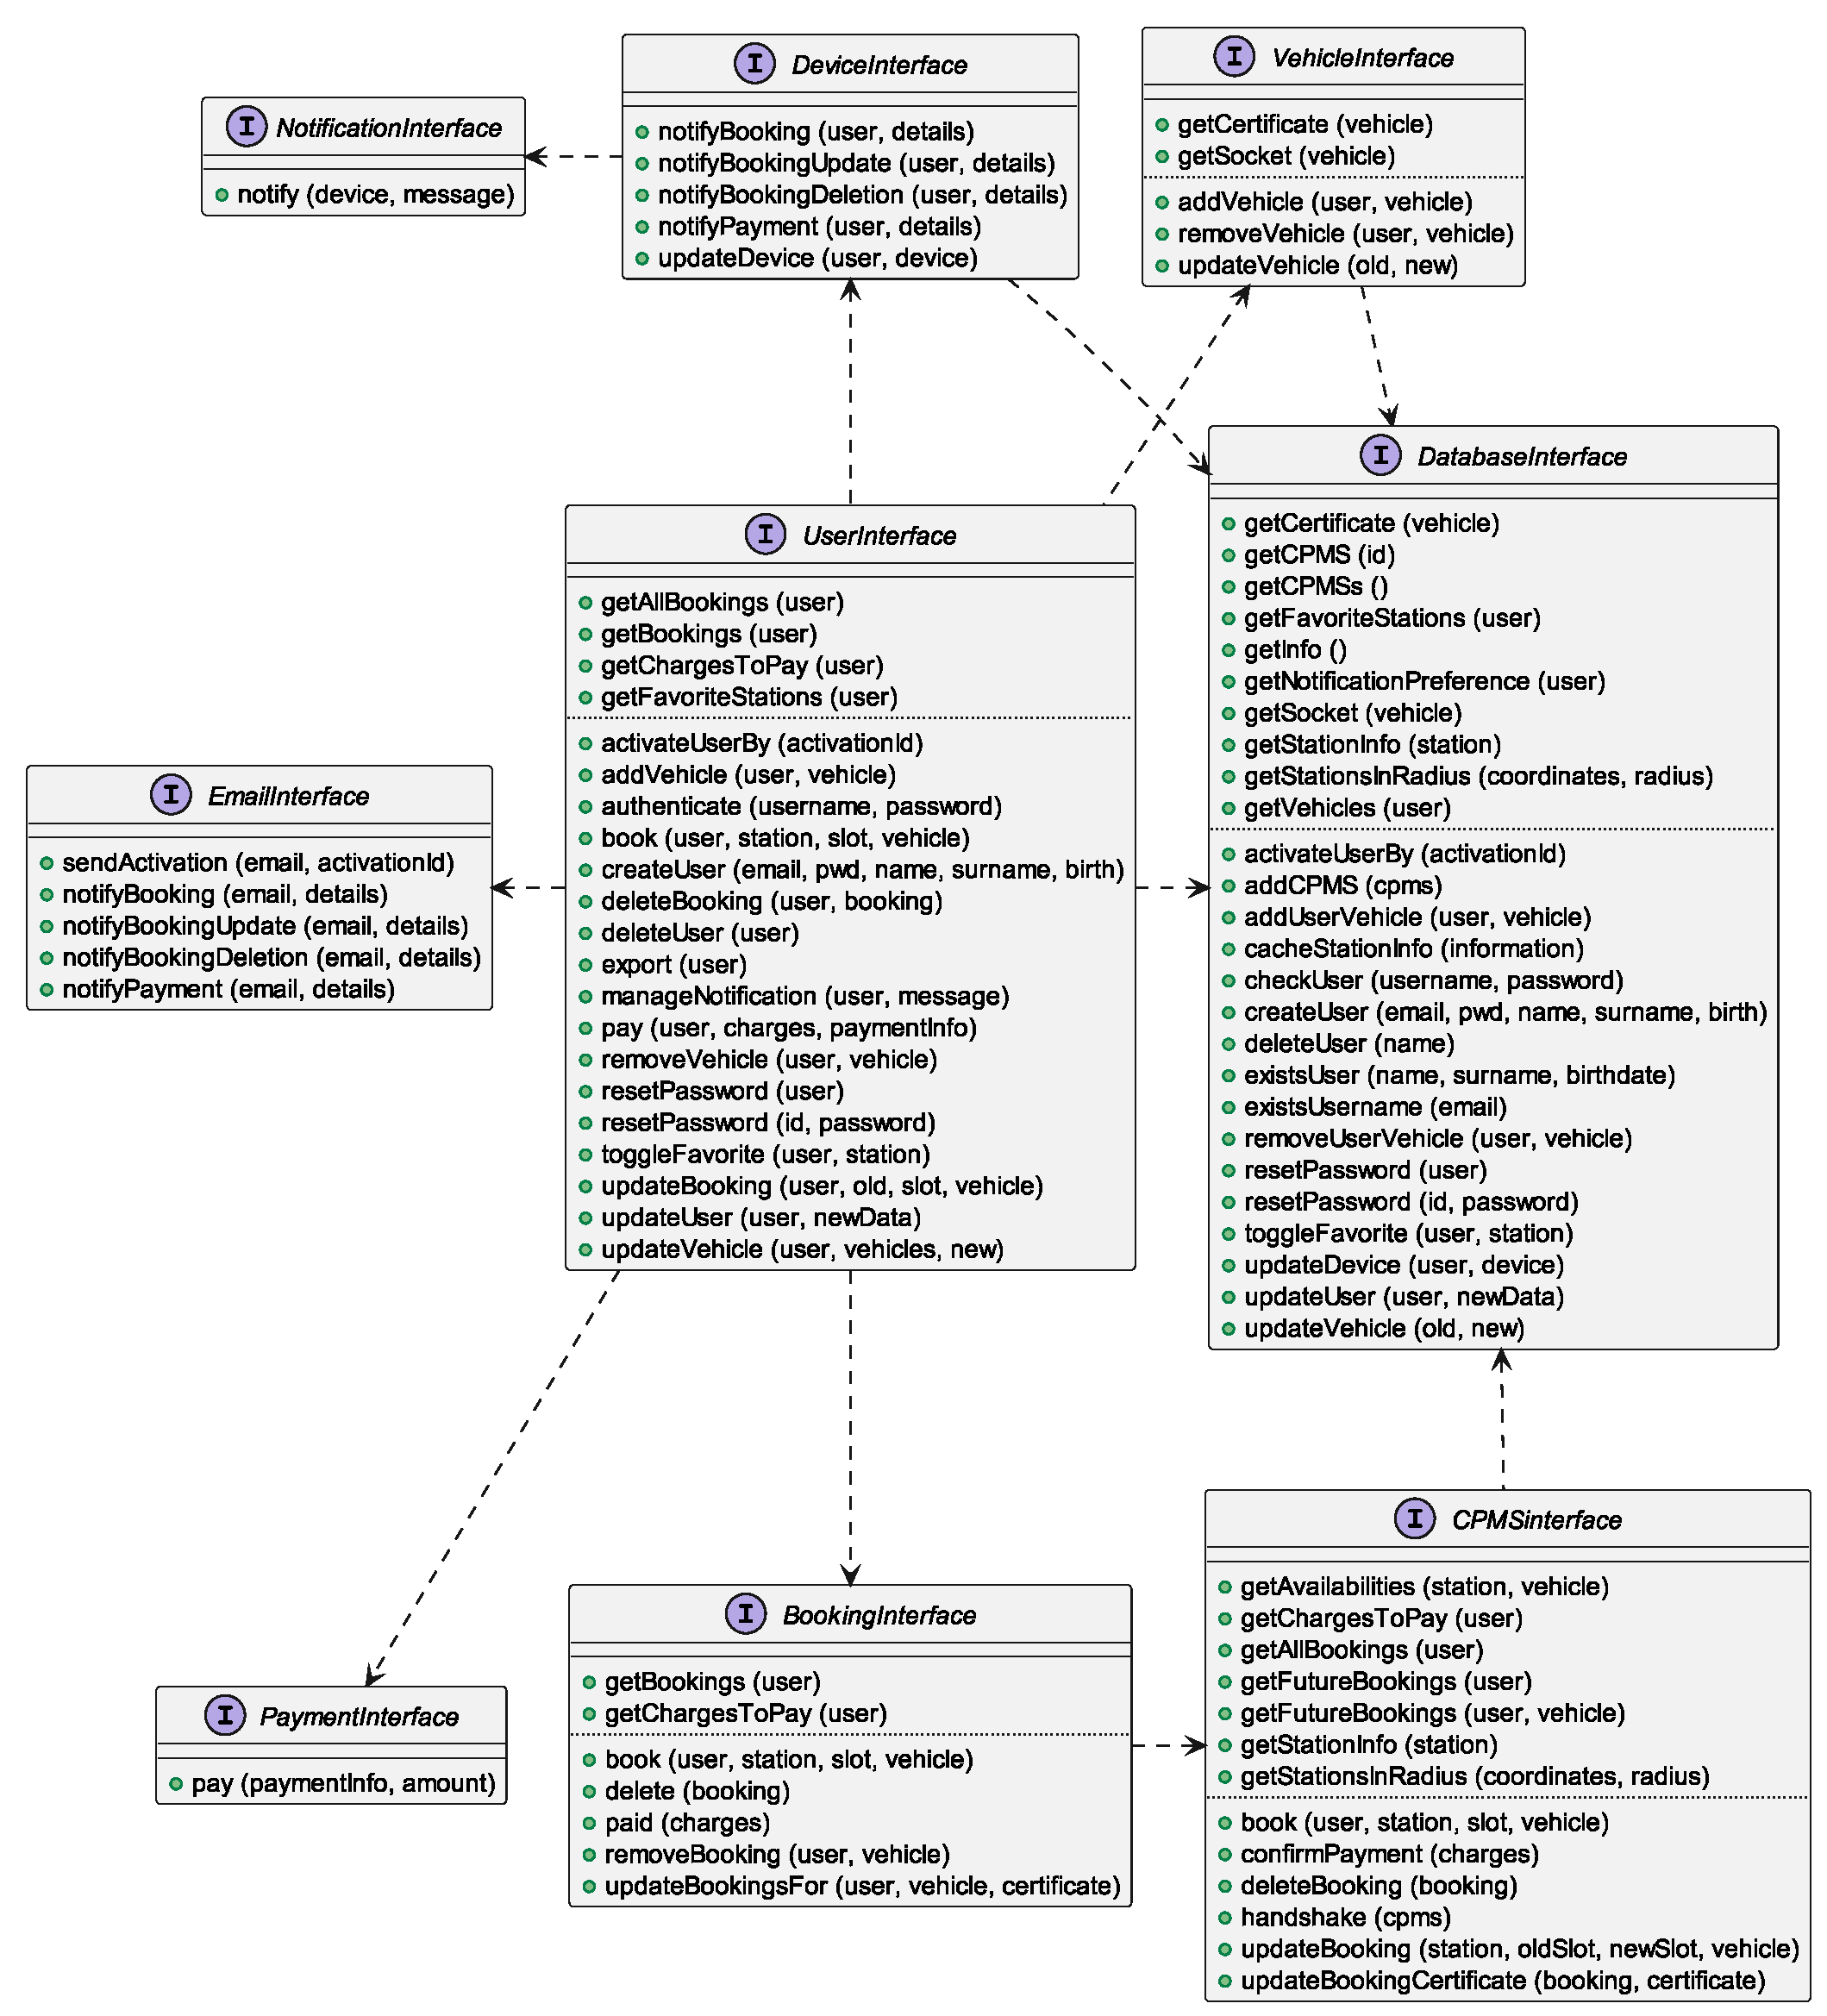
\includegraphics[width=0.84\columnwidth]{./images/interfaces/emsp}
    \caption{internal interfaces of the eMSP system and their functions.}
\end{figure}

\subsection{CPMS}

\figureref{figure:interface:cpms} depicts the internal interfaces of the CPMS system. The functions inside the interfaces cover all functionalities implemented by the CPMS system and/or needed by the eMSP system, and can be improved for future versions of these systems.\medskip

Most interfaces in the CPMS systems make use of the \texttt{DatabaseInterface}, to write to durable storage all changes happening to the system. This is done to be able to recover quickly in case of failures, in order to guarantee the promised availability. Most functions offered in components' interfaces make use of the same function or a similar function offered by the \texttt{DatabaseInterface}, since the \texttt{DatabaseHandler} is the only component that directly communicates with the database.

\begin{figure}[h!]
    \centering
    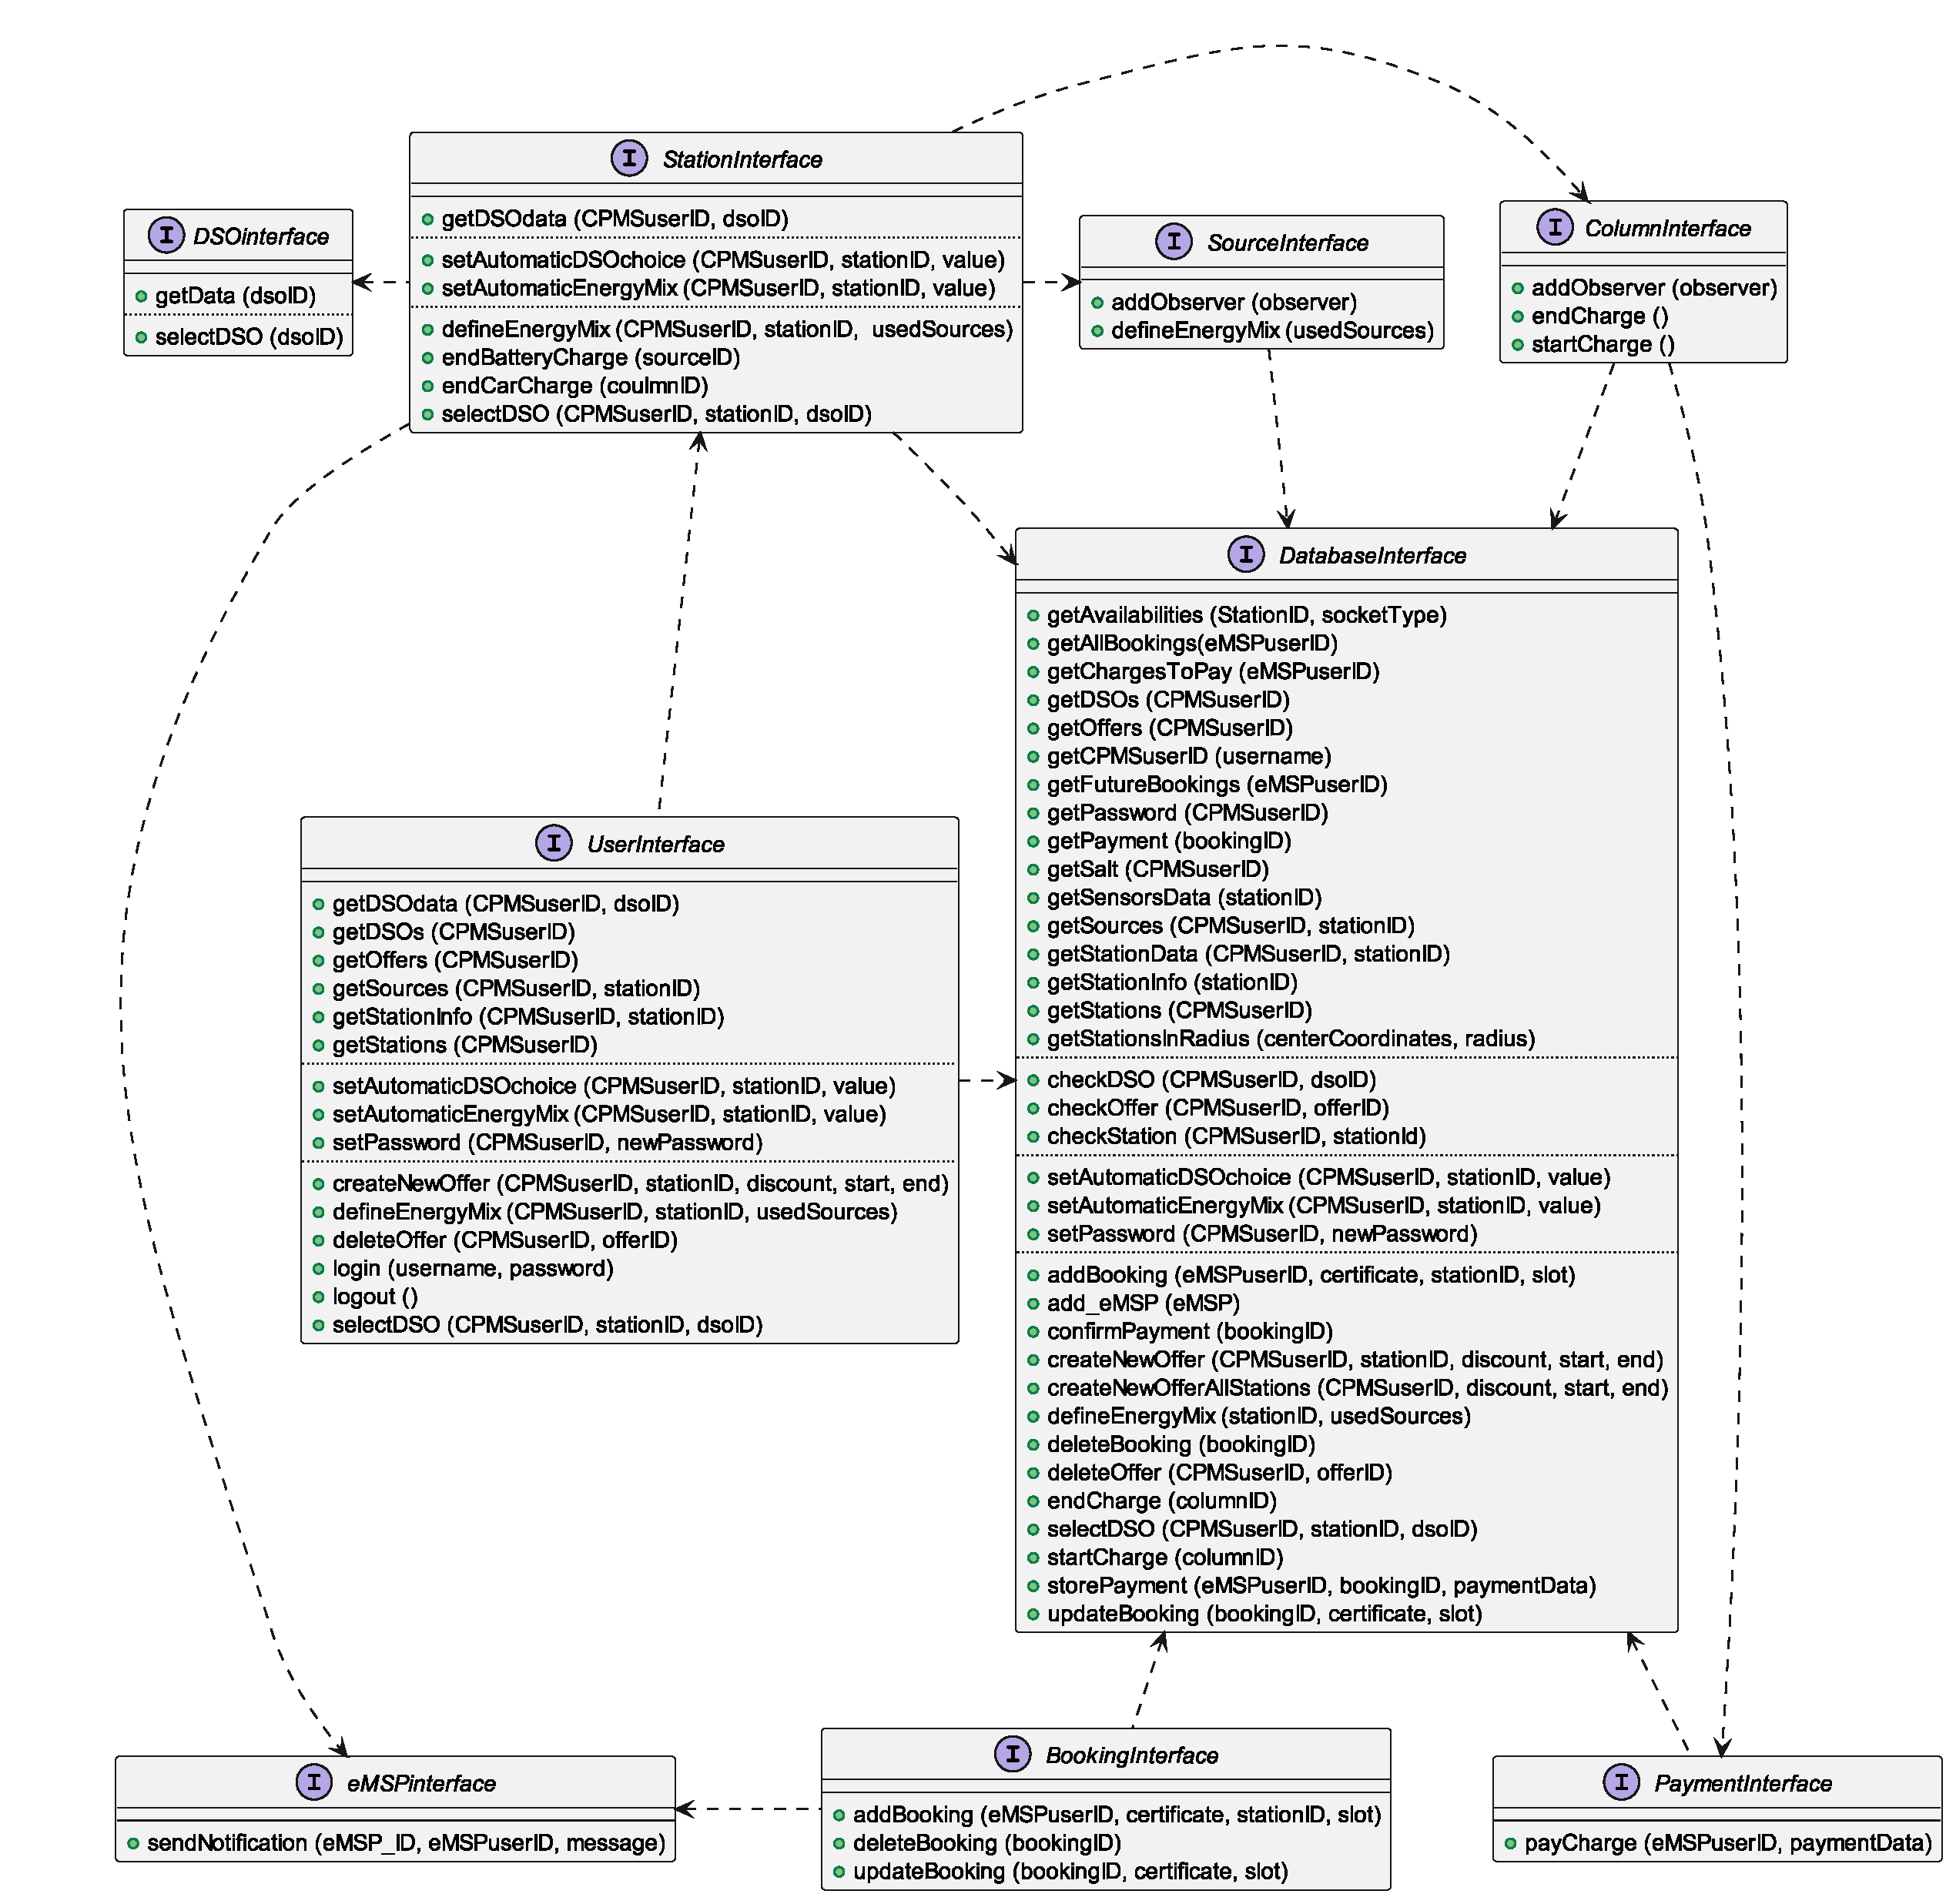
\includegraphics[width=\columnwidth]{./images/interfaces/cpms}
    \caption{internal interfaces of the CPMS system and their functions.}
    \label{figure:interface:cpms}
\end{figure}

\pagebreak

\section{Runtime view} \label{view:runtime}

Here are presented some important actions the user or the system does and how the various components are activated through which function calls in order to perform the required actions.\medskip

Every time \doublequotes{consumer} or \doublequotes{user} appears in a UML diagram, it's intended that s/he is interacting with the application or web page that interacts with the system.\medskip

For the sake of simplicity, many data checks and the opening of the application or web page, according to the use case, are not illustrated, but they are present in the system. Moreover, some cases are not depicted here:
\begin{itemize}
    \item \textit{Notification preference}: the user is asked to choose between in-app notifications or email ones after his first login. Furthermore, the user can change this preference at any time under his/her profile.
    \item \textit{Logout}: simply removes the token from the client.
    \item \textit{Password change}: it works like most of the password changes implemented nowadays. The first option is that the user clicks on the \doublequotes{Forgot password?} link, receives an email with the link for changing it, and changes the password. The second one is that s/he goes to the user's details page and changes the password directly from there. In both cases, s/he has to log back in on all his/her connected devices.
\end{itemize}
Also, even if it's not specified in the diagrams, if any component fails, the user is notified and the action is automatically aborted, reverting its state to the original one. The same happens in case of user's network failures (which are \doublequotes{detected} through a timeout).

\subsection{eMSP}

\paragraph{Registration} The user registers into the system providing the required data through a dedicated form and his/her email address which is then used for sending the activation link and eventual notifications.

\begin{figure}[h!]
    \centering
    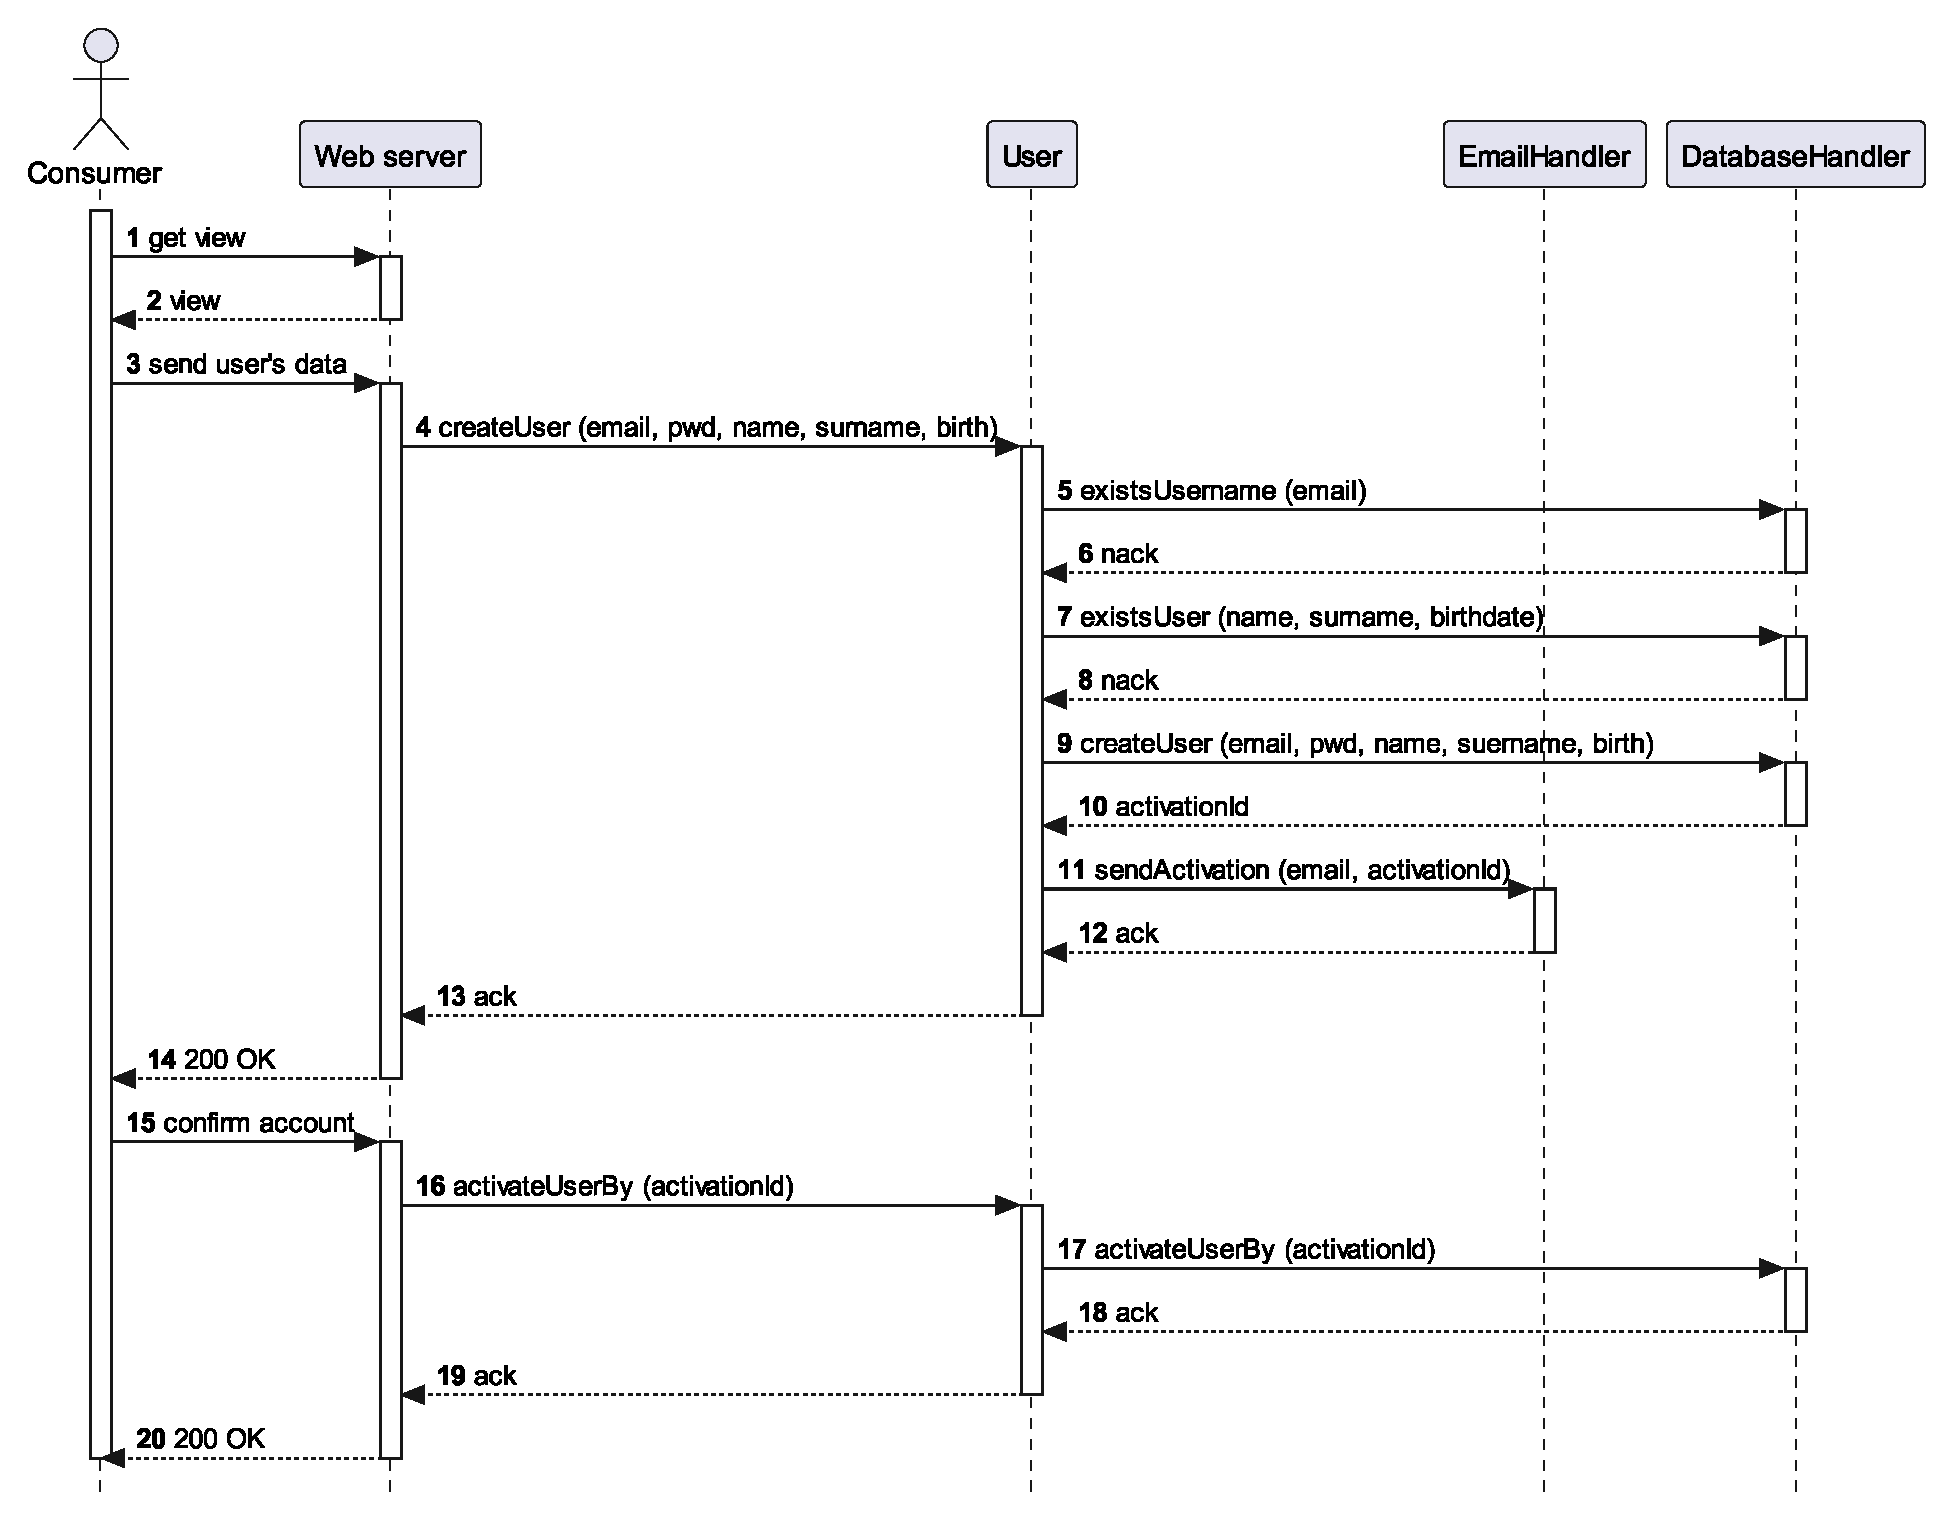
\includegraphics[width=\columnwidth]{./images/sequences/emsp/registration}
    \caption{registration of the eMSP user (consumer).}
\end{figure}

\pagebreak

\paragraph{Login} The user logs into the system, which recognizes him/her and sends back a signed JWT for future actions on the system, like booking charges. This token is properly checked on every request by the web server.

\begin{figure}[h!]
    \centering
    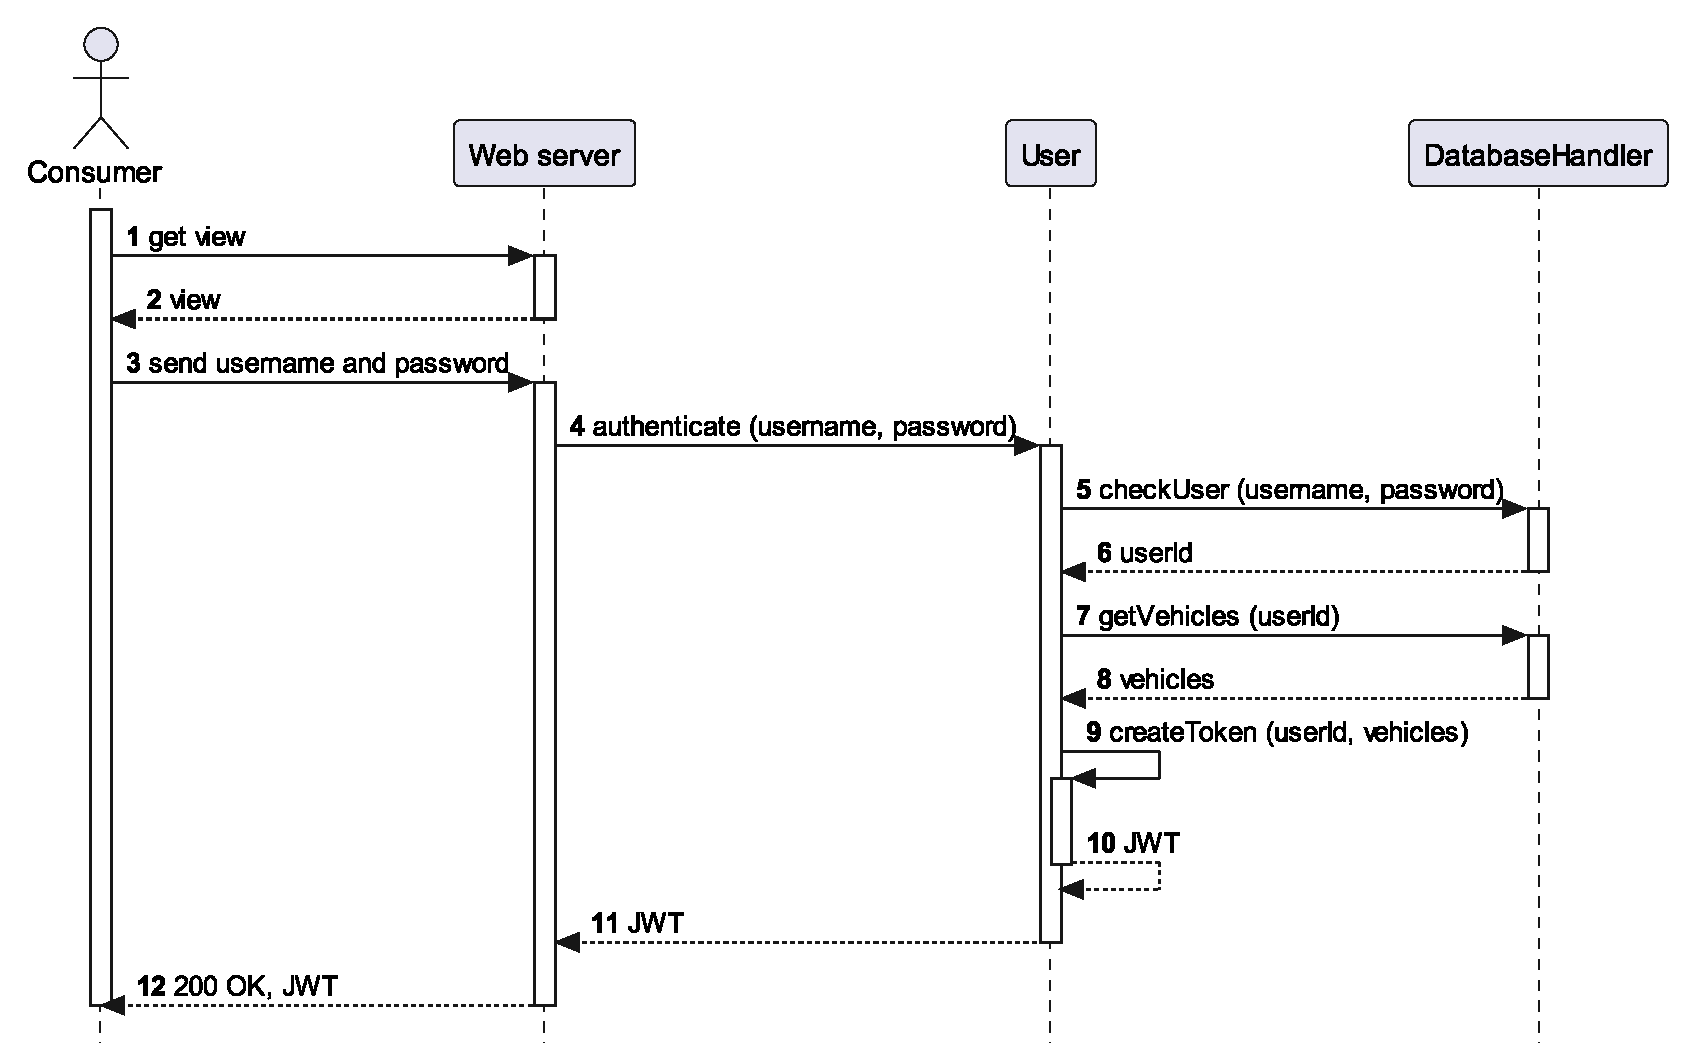
\includegraphics[width=\columnwidth]{./images/sequences/emsp/login}
    \caption{login of the eMSP user (consumer).}
\end{figure}

\paragraph{Mark/unmark a station as favorite} The user marks or unmarks any wanted charging station as favorite. The following diagram shows how the stations can be found thanks to this system.

\begin{figure}[h!]
    \centering
    
\includegraphics[width=0.9\columnwidth]{./images/sequences/emsp/favorite}
    \caption{the user marks/unmarks a station as \doublequotes{favorite}.}
\end{figure}

\pagebreak

\paragraph{Look for nearby stations} The user looks for a charging station, either by searching a location or by using a geolocalization service. In any case it's possible to use the map or the list view.

\begin{figure}[h!]
    \centering
    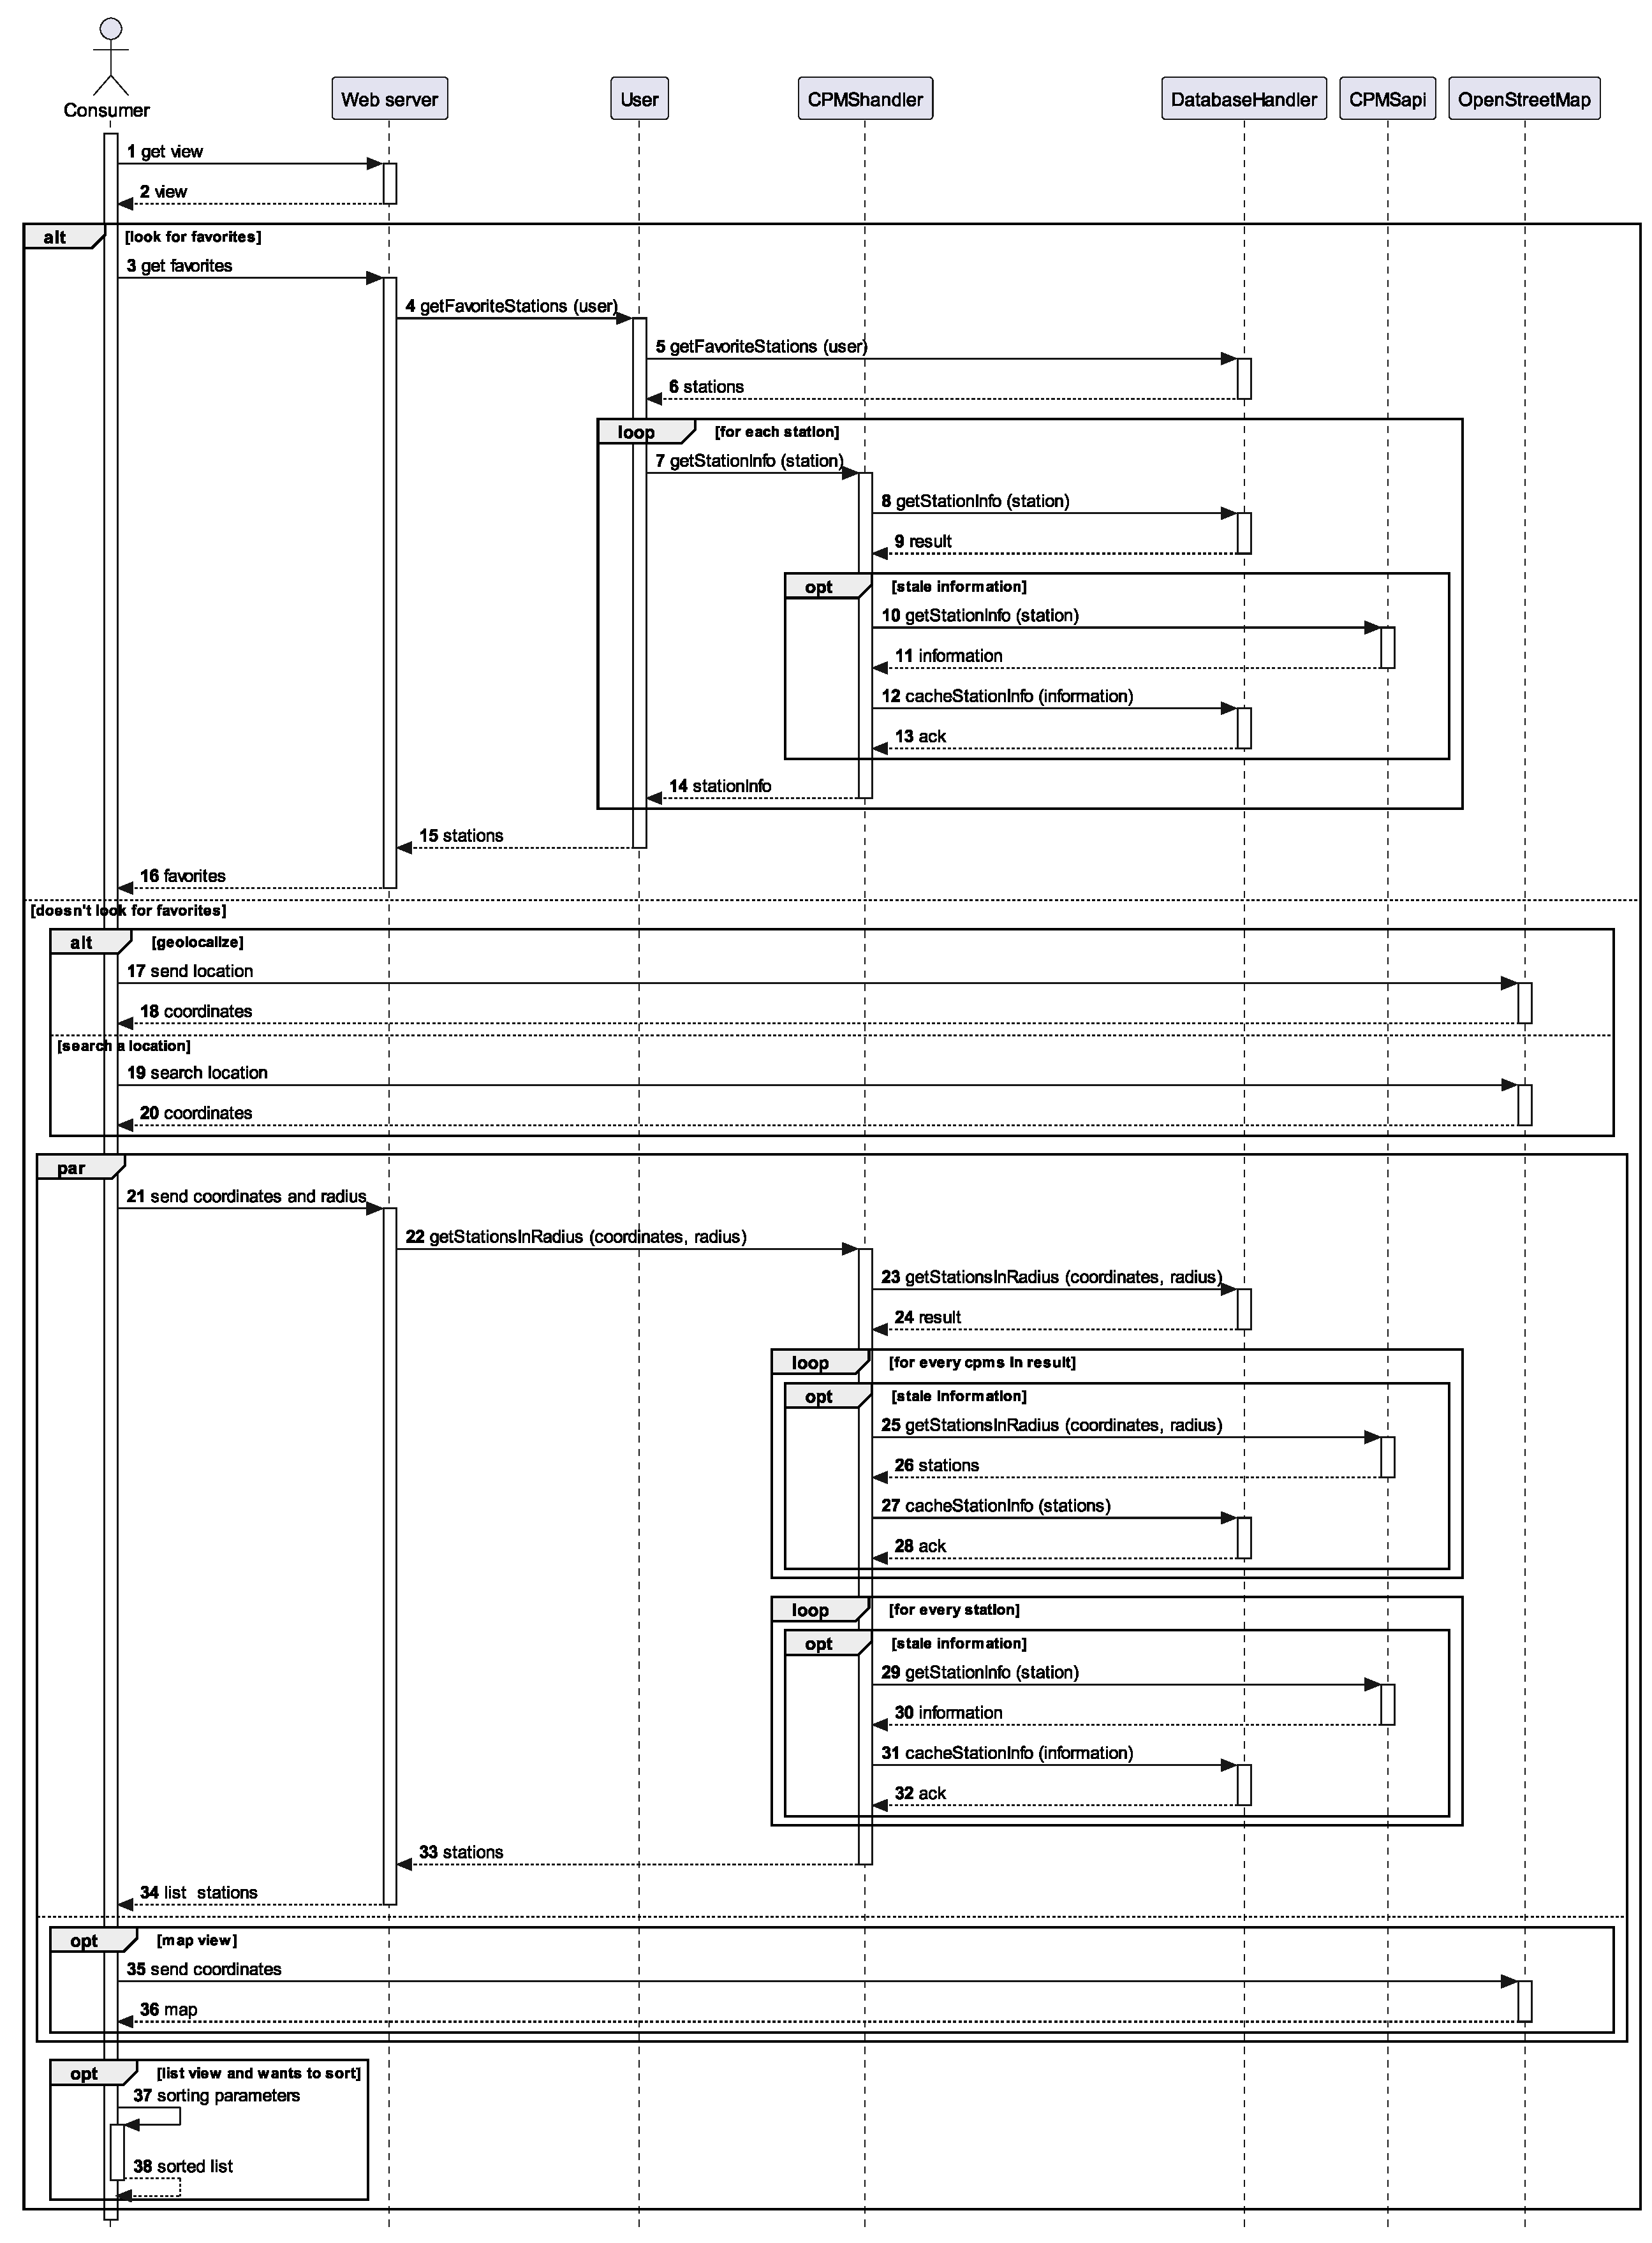
\includegraphics[width=\columnwidth]{./images/sequences/emsp/lookup}
    \caption{the user looks for a charging station.}
\end{figure}

\pagebreak

\paragraph{Book a charge} After finding a suitable station (which is depicted in the previous diagram), the user can book a charge by providing the required data to the system.

\begin{figure}[h!]
    \centering
    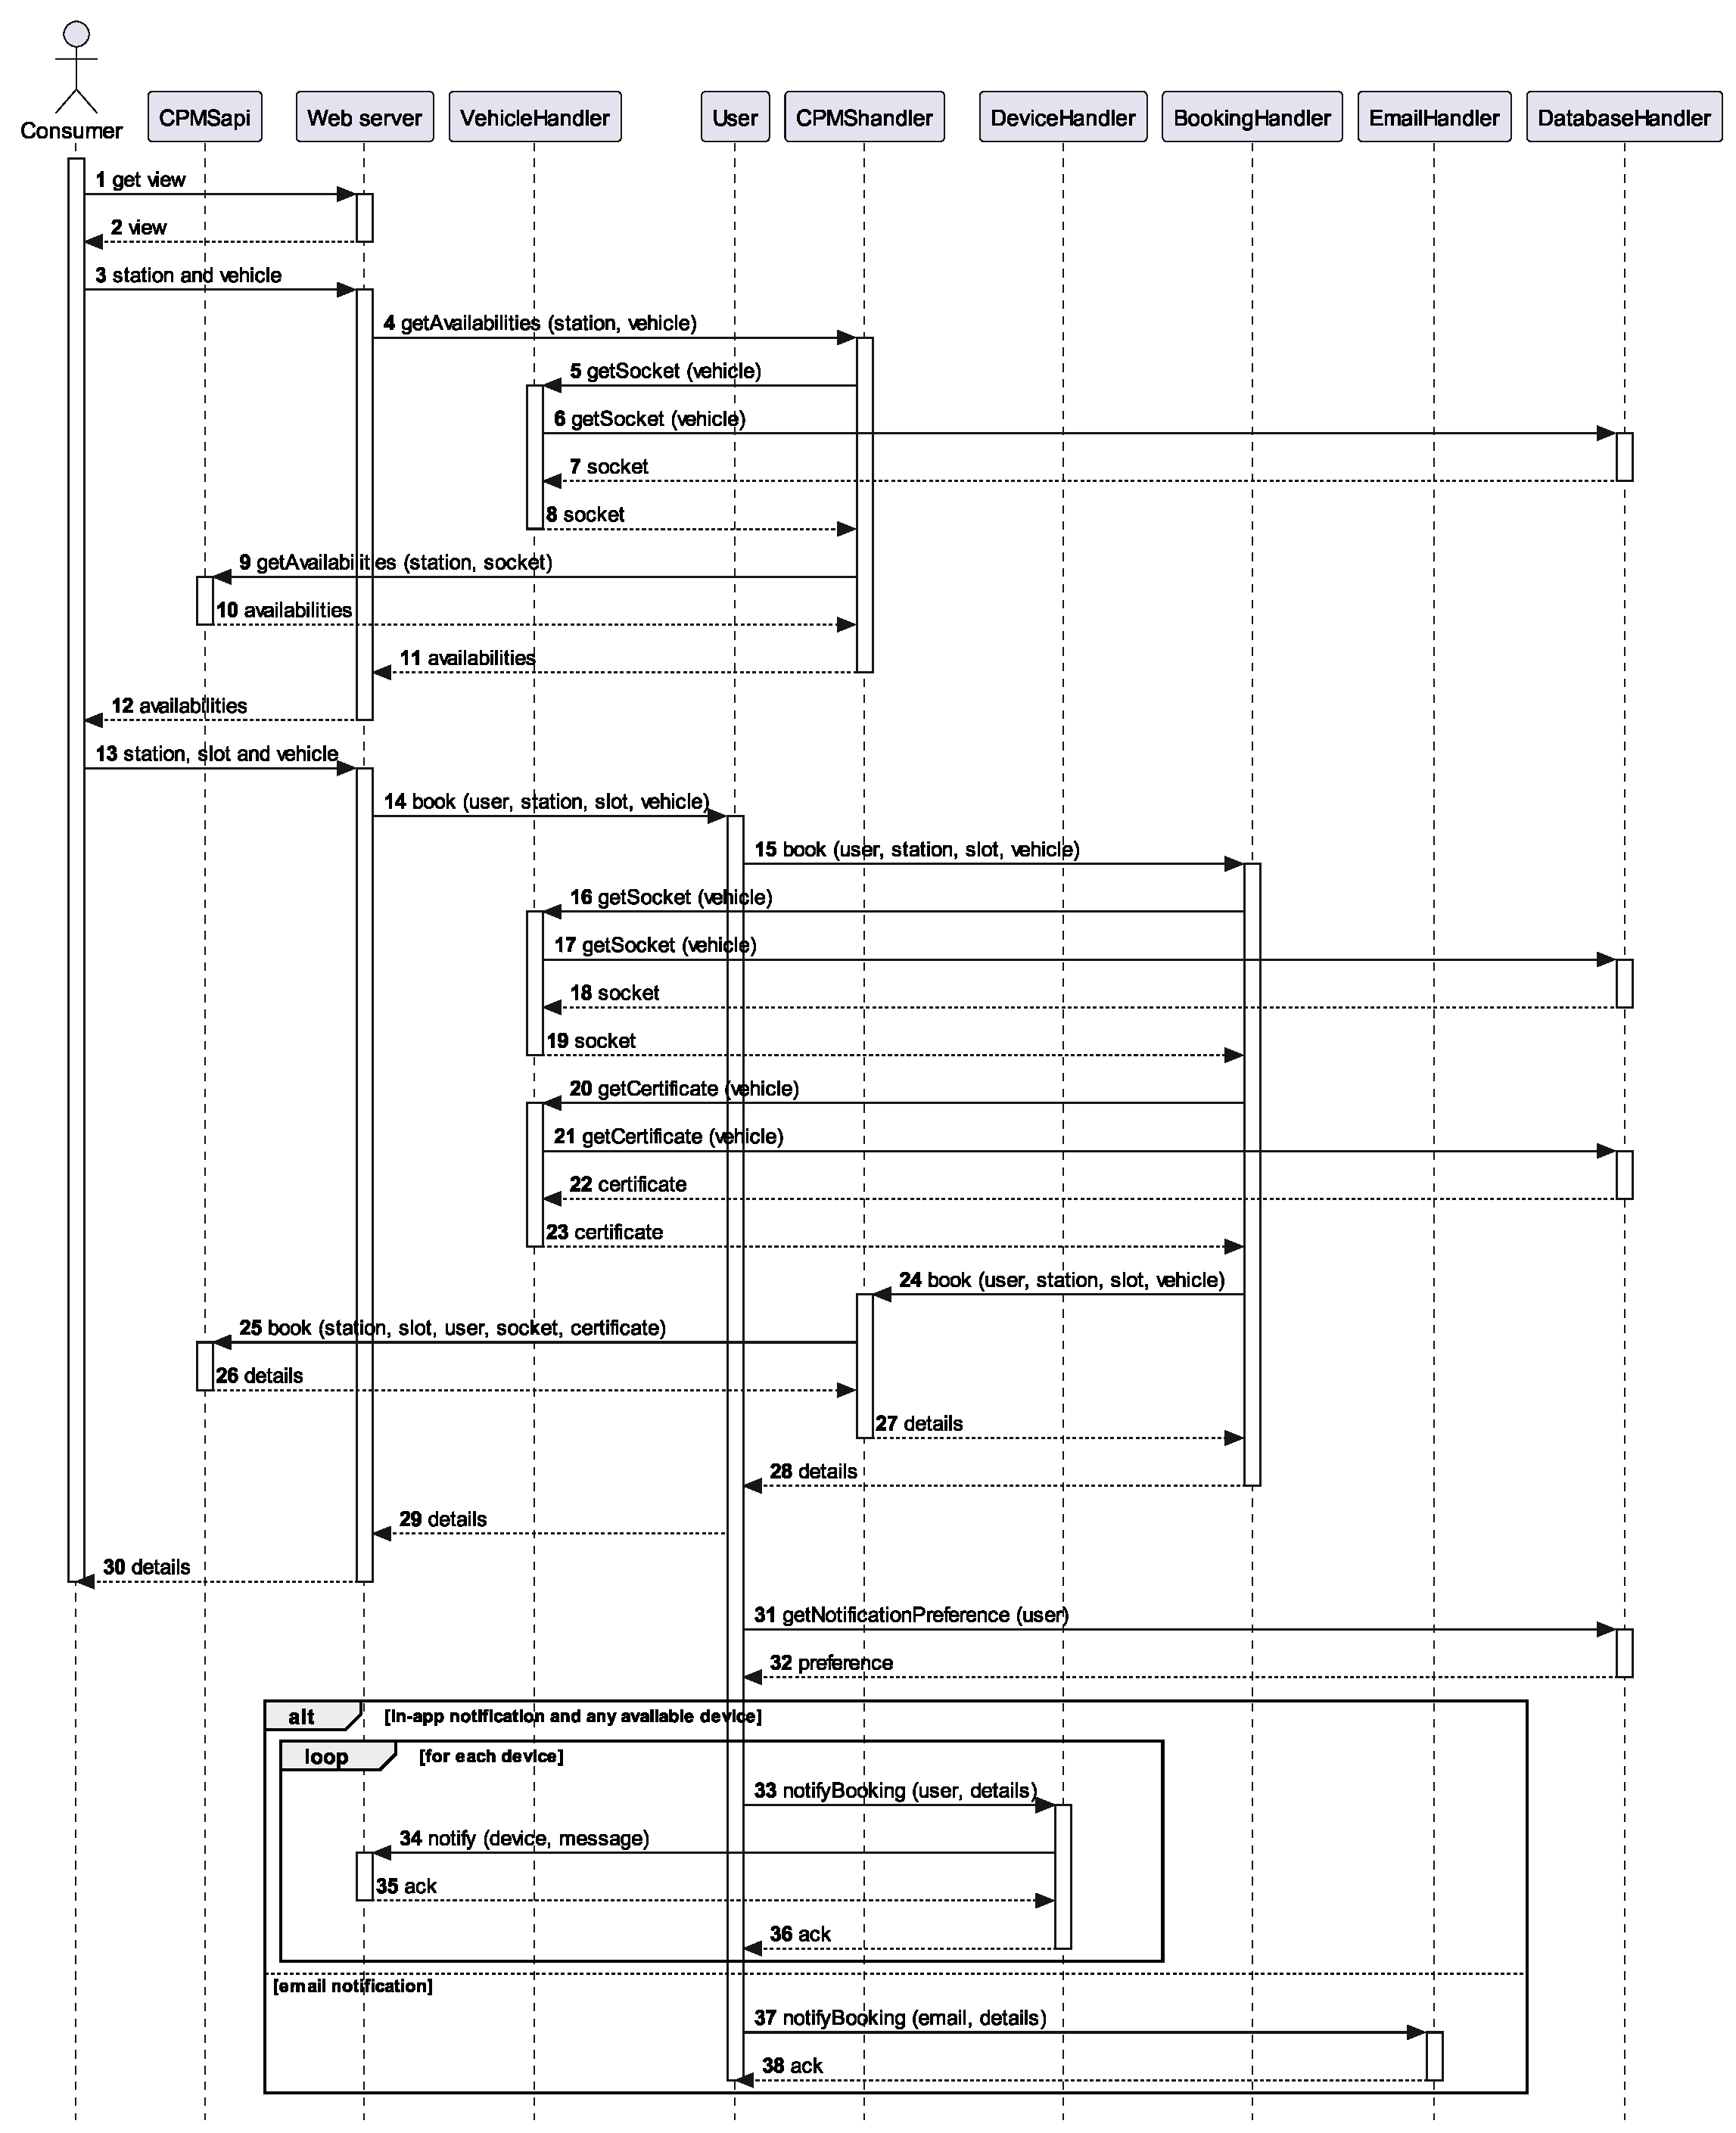
\includegraphics[width=\columnwidth]{./images/sequences/emsp/book_add}
    \caption{the user books a charge.}
\end{figure}

\pagebreak

\paragraph{Edit a reservation} If the user needs to, it's possible to modify an already existing booked charge for the same station, providing the required data.

\begin{figure}[h!]
    \centering
    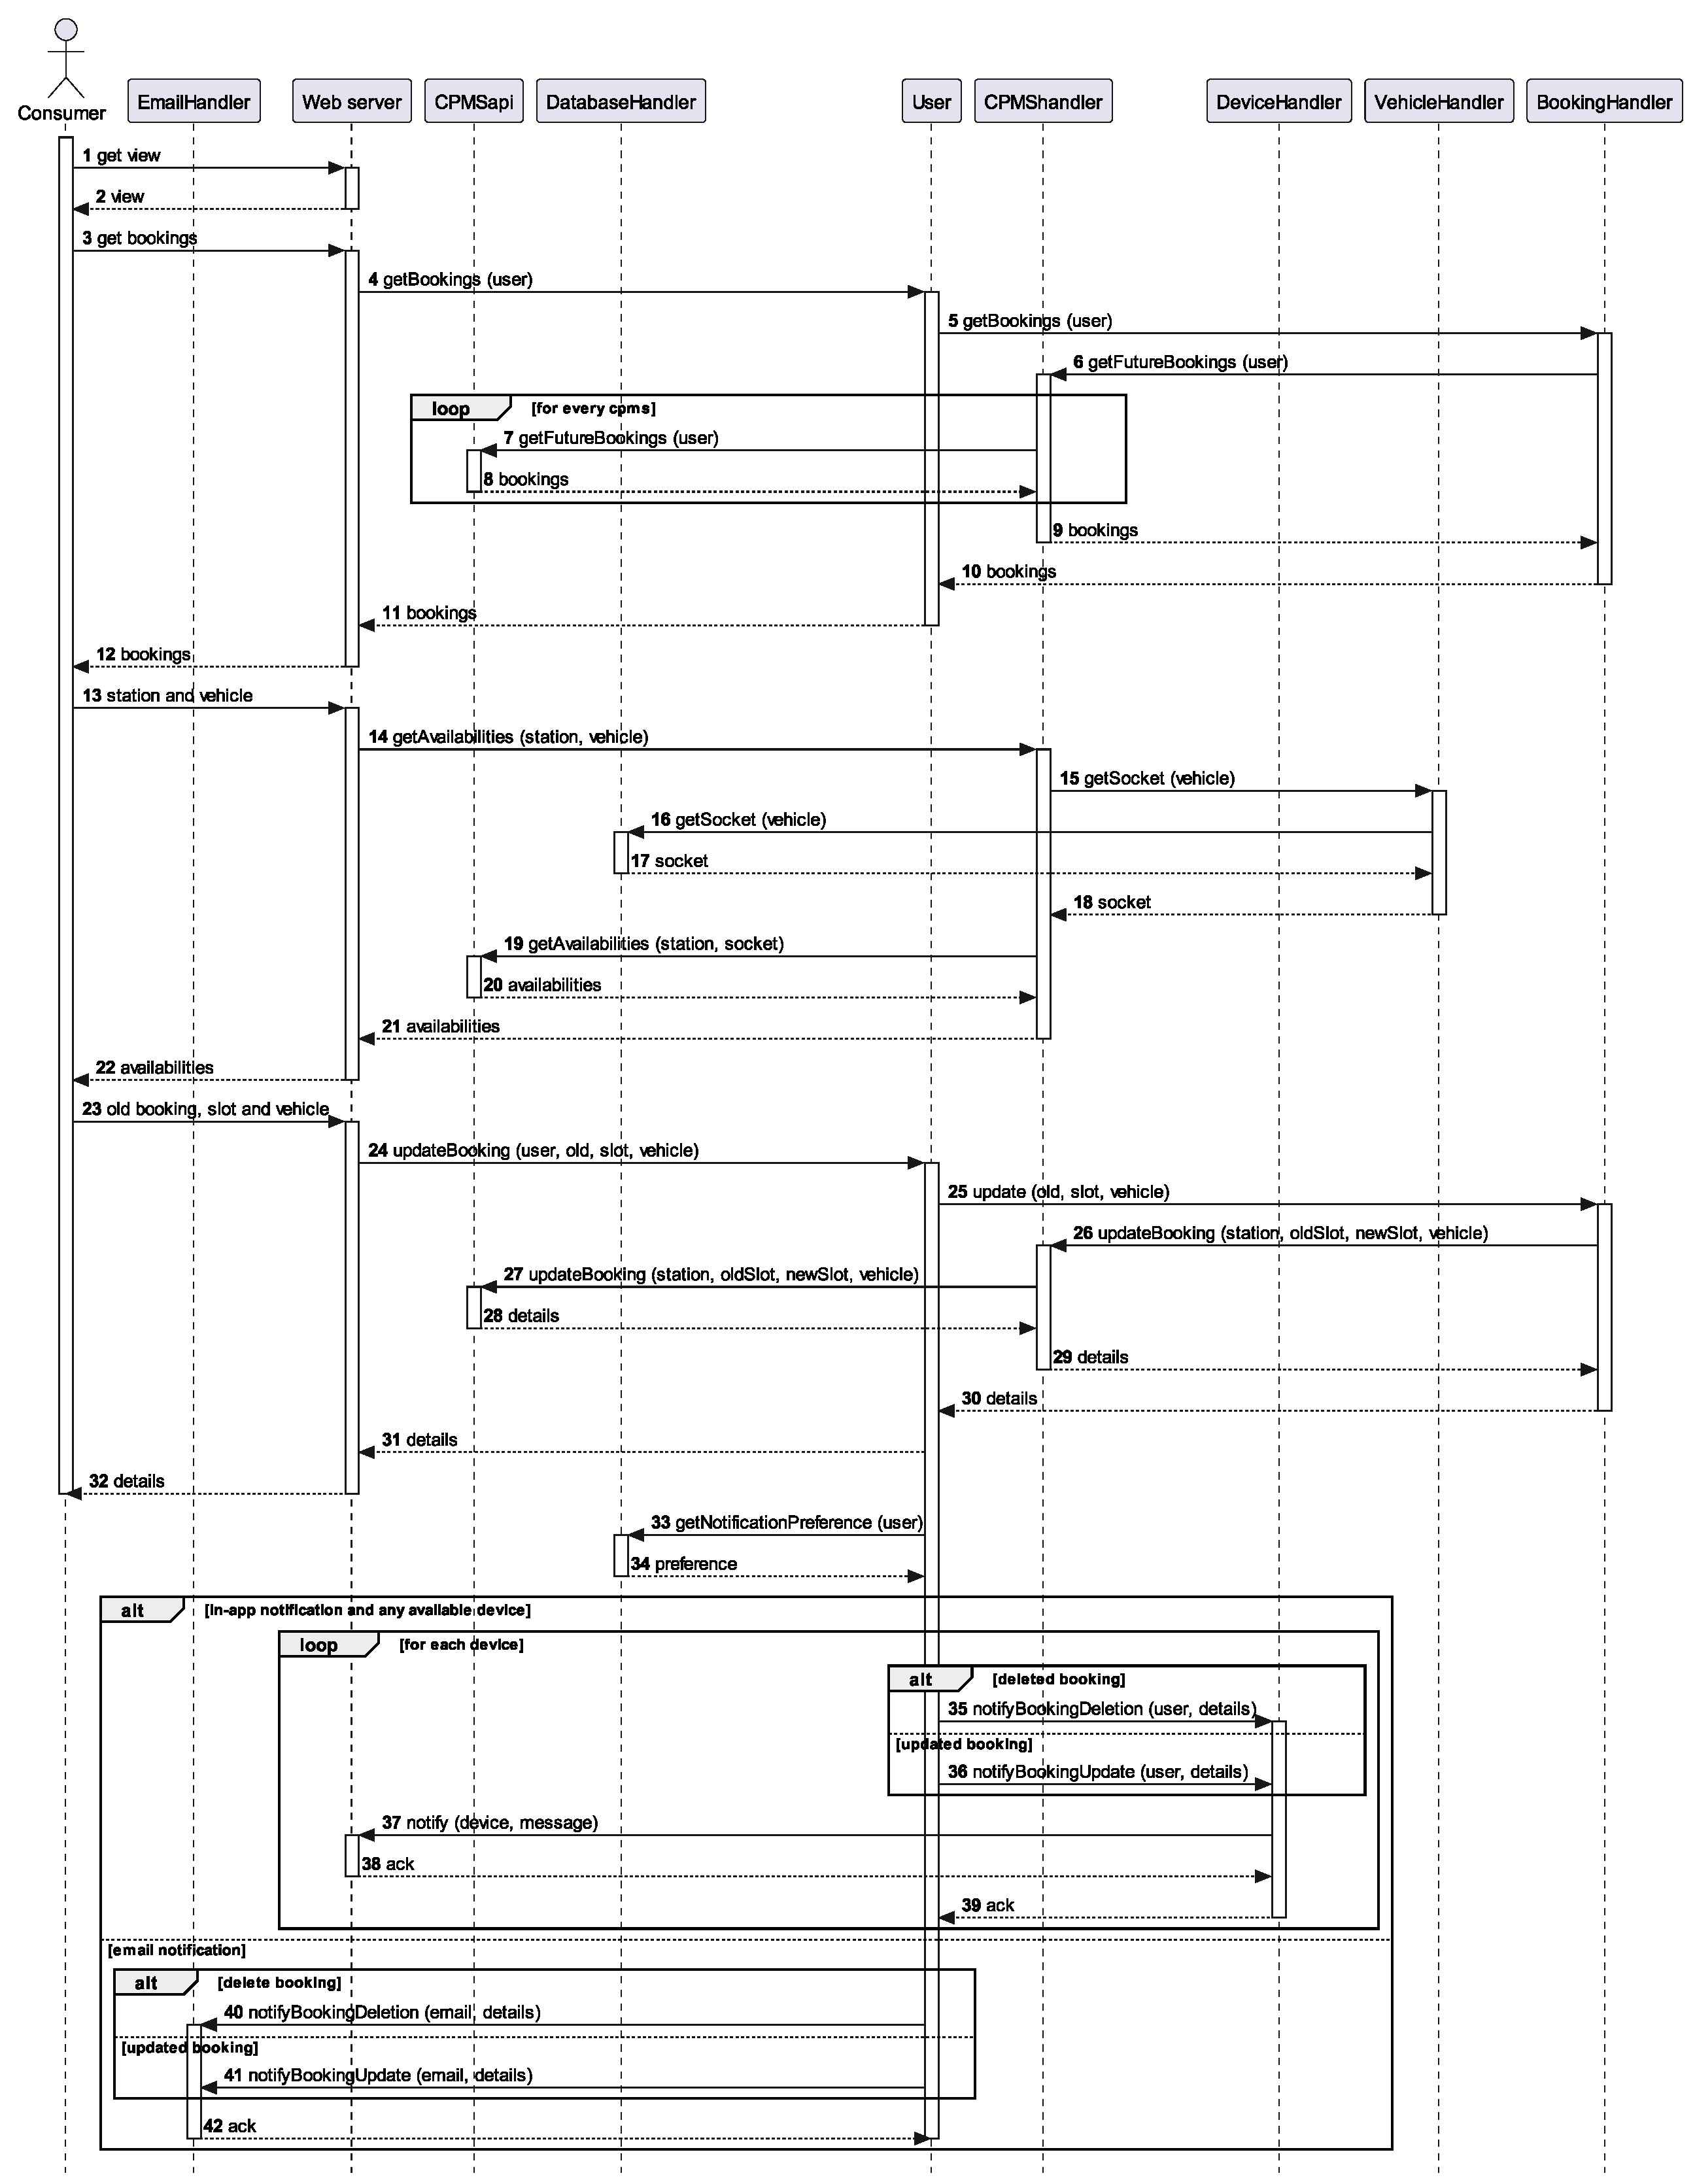
\includegraphics[width=\columnwidth]{./images/sequences/emsp/book_edit}
    \caption{the user edits a booked charge.}
\end{figure}

\pagebreak

\paragraph{Delete a reservation} If the user needs to, it's possible to delete a previously booked charge unless it's in the past.

\begin{figure}[h!]
    \centering
    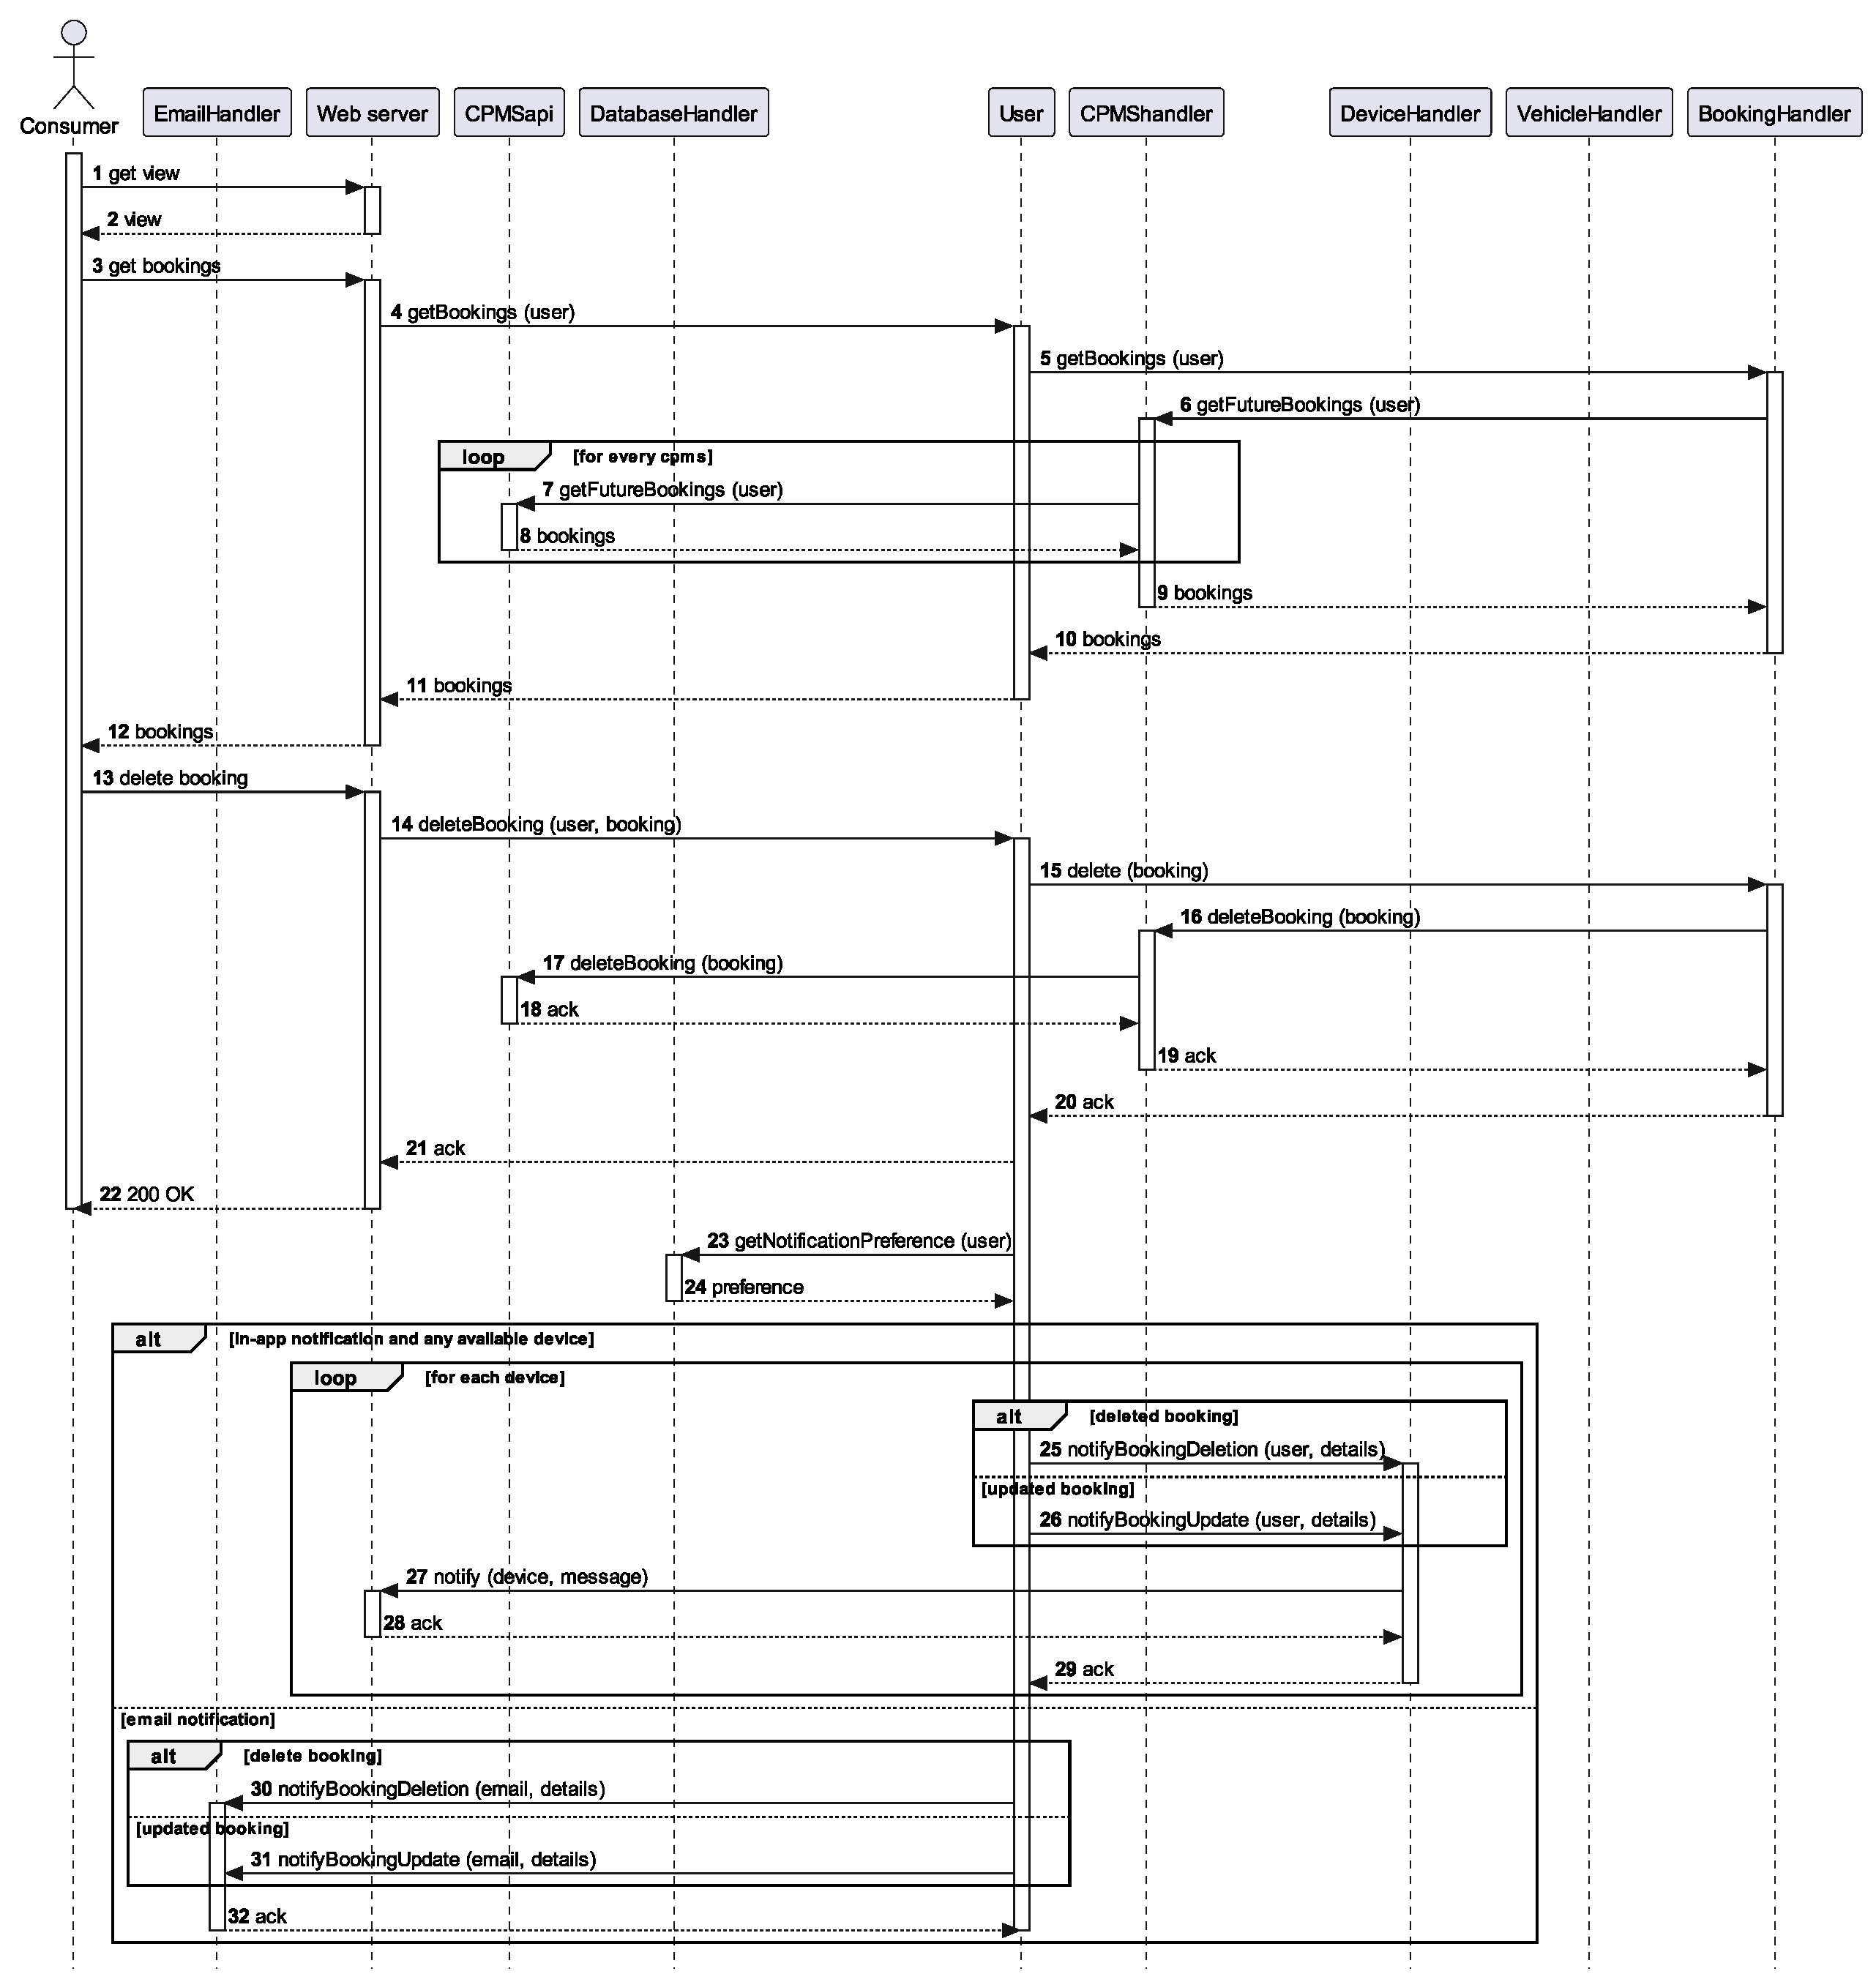
\includegraphics[width=\columnwidth]{./images/sequences/emsp/book_delete}
    \caption{the user removes a booked charge.}
\end{figure}

\pagebreak

\paragraph{Pay for the obtained services} After a charge is completed, the user can pay the charge. If more than one charge needs to be paid, they are aggregated into one single payment.

\begin{figure}[h!]
    \centering
    
\includegraphics[width=\columnwidth]{./images/sequences/emsp/payment}
    \caption{the user pays for the charges.}
\end{figure}

\pagebreak

\paragraph{Editing of a vehicle} The user can edit at any time his/her vehicles. If also the vehicle's certificate is changed, the system automatically updates all future reservations by telling the CPMSs which is the new certificate for the charge.

\begin{figure}[h!]
    \centering
    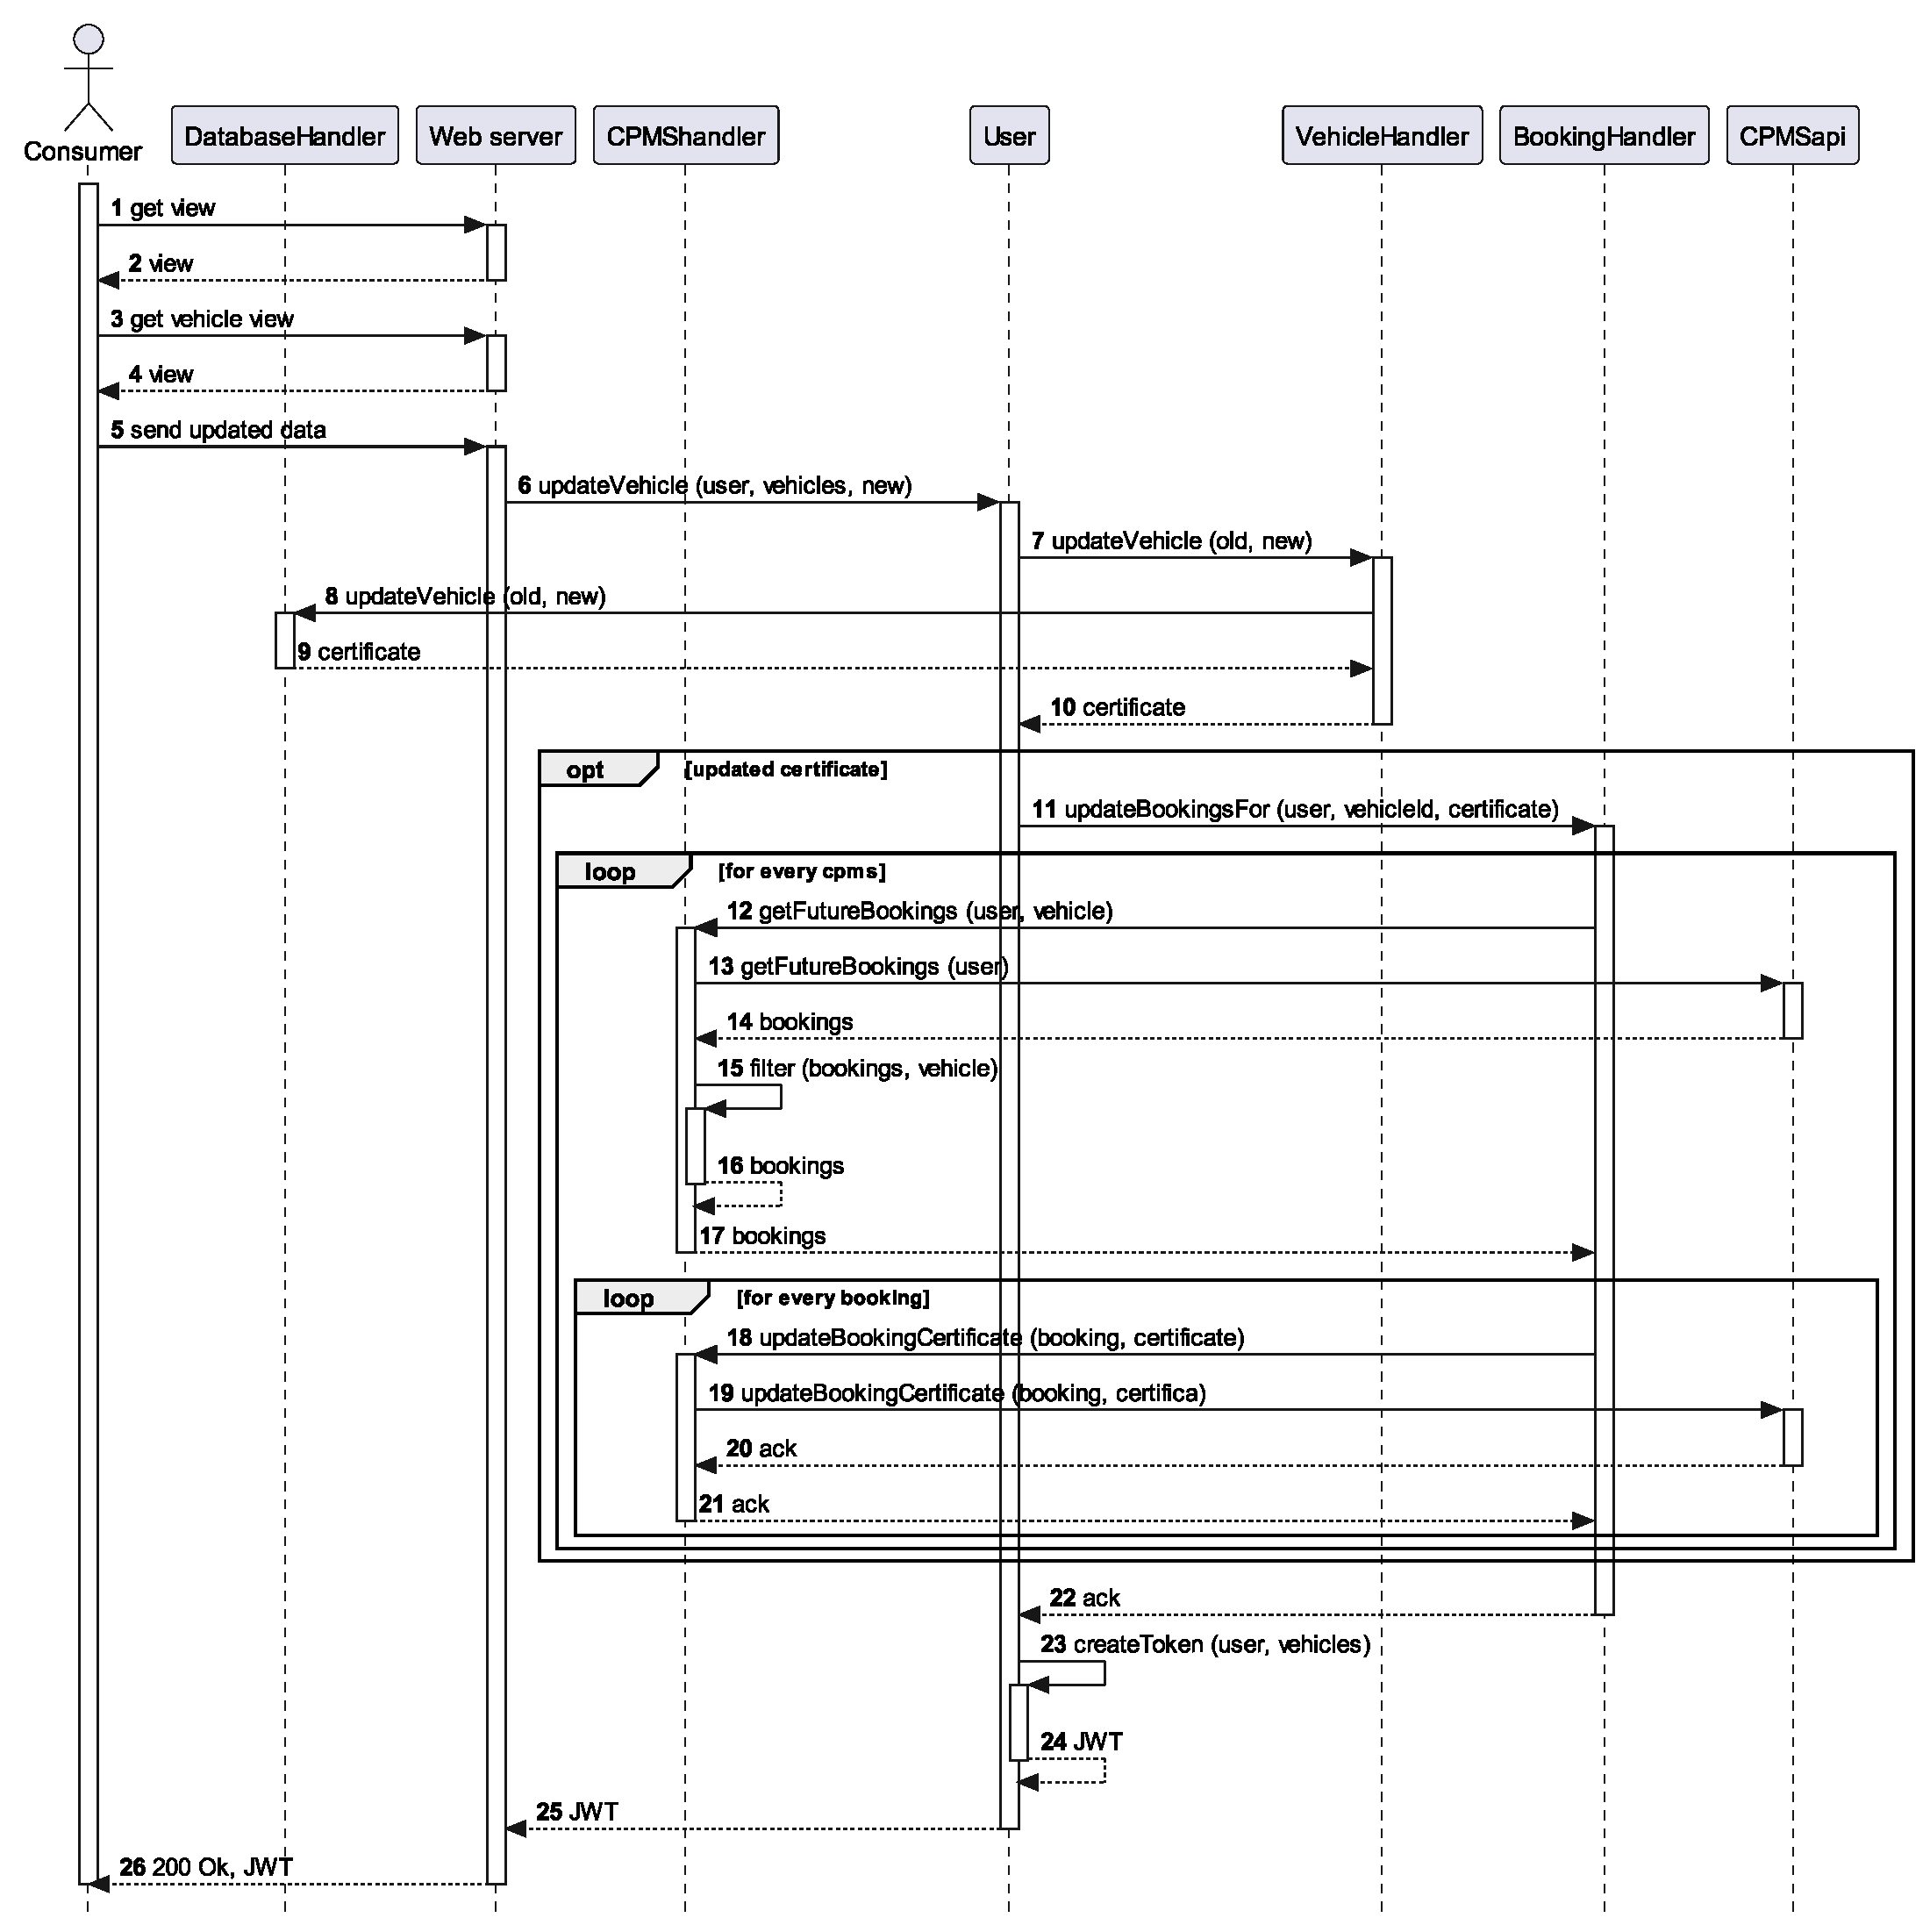
\includegraphics[width=\columnwidth]{./images/sequences/emsp/vehicle_edit}
    \caption{the user edits one of his/her vehicles.}
\end{figure}

\pagebreak

\paragraph{Deletion of a vehicle} The user can delete at any time his/her vehicles. Every time a vehicle is removed, the system automatically deletes all future reservations for that vehicle on every CPMS.

\begin{figure}[h!]
    \centering
    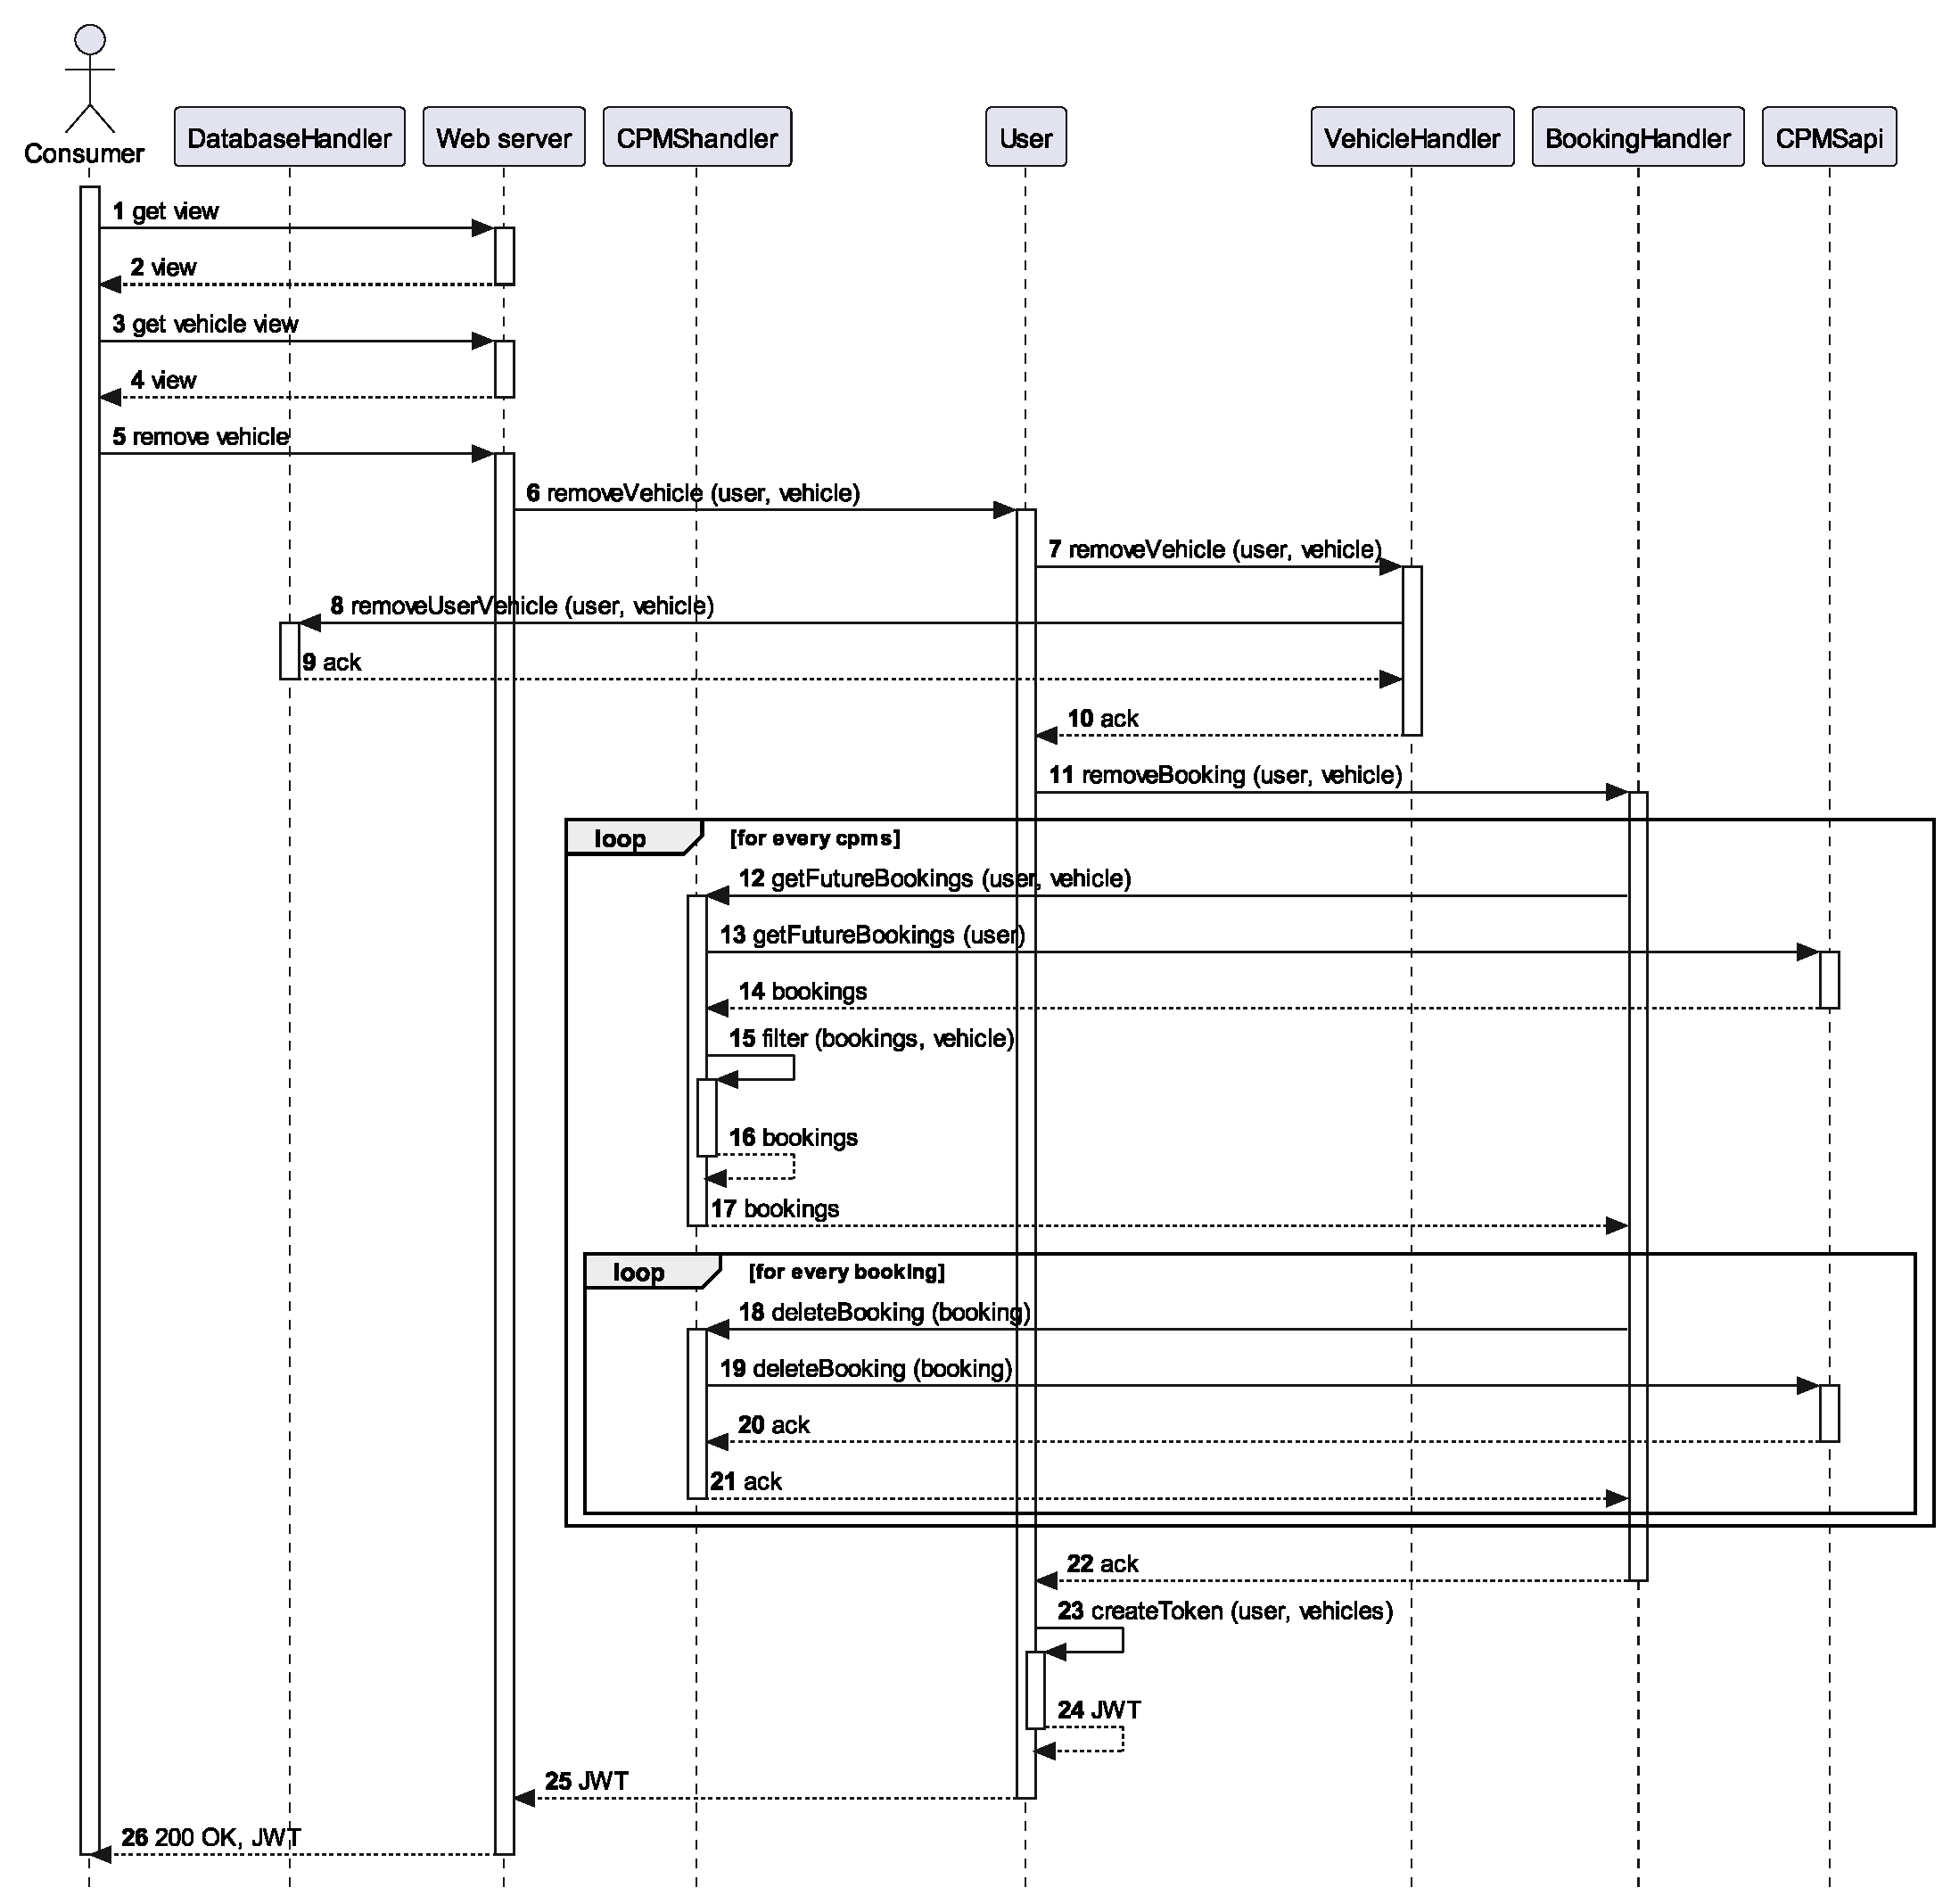
\includegraphics[width=\columnwidth]{./images/sequences/emsp/vehicle_delete}
    \caption{the user removes one of his/her vehicles.}
\end{figure}

\pagebreak

\paragraph{Addition of a new vehicle} The user adds a new vehicle to the system by providing the required data and its certificate.

\begin{figure}[h!]
    \centering
    \includegraphics[width=\columnwidth]{./images/sequences/emsp/vehicle_add}
    \caption{the user adds a new vehicle.}
\end{figure}

\paragraph{Other functions} In the \reference{view:interfaces} section there are some eMSP functions that are not used in these sequence diagrams, in particular:
\begin{itemize}
    \item \texttt{deleteUser (user)} \textit{from} \texttt{UserInterface} \textit{and} \texttt{DatabaseInterface}: if the user doesn't have any pending payment, the system removes all his/her data from the system and all the future bookings.
    \item \texttt{export (user)} \textit{from} \texttt{UserInterface}: allows the user to export all his/her data collected by the eMSP and the CPMS, according to the GDPR.
    \item \texttt{getAllBookings (user)} \textit{from} \texttt{CPMSinterface} \textit{and} \texttt{UserInterface}: retrieves all the booking for that user on every connected CPMS.
    \item \texttt{resetPassword (user)} \textit{and} \texttt{resetPassword (id, link)} \textit{from} \texttt{UserInterface} \textit{and} \linebreak \texttt{DatabaseInterface}: these two methods allow the user to reset his/her access password by proving the email address used for logging in. The system sends the user an email with the link for changing it.
    \item \texttt{updateUser (user, newData)} \textit{from} \texttt{UserInterface}: allows the user to update all his/her data, including the password.
    \item \texttt{updateDevice (user, device)} \textit{from} \texttt{DeviceInterface} \textit{and} \texttt{DatabaseInterface}: even if it's not presented in the diagrams, it's called on every request for keeping updated the list of devices of the user, which are automatically cleaned up after a while if unused.
    \item \texttt{handshake (cpms)} \textit{from} \texttt{CPMSinterface} \textit{and} \texttt{addCPMS (cpms)} \textit{and} \texttt{getInfo ()}\footnote{This function (\texttt{getInfo ()}) allows to retrieve all the eMSP's information that need to be sent to the newly connected CPMS.} \textit{from} \linebreak \texttt{DatabaseInterface}: these functions allow the system to conncet to a newly discovered CPMS and to store it's information into the database.
    \item \texttt{getCPMS (id)} \textit{and} \texttt{getCPMSs ()} \textit{from} \texttt{DatabaseInterface}: allow retrieving data about a specific CPMS or about every connected one.
\end{itemize}

\vfill

\pagebreak

\subsection{CPMS}

\paragraph{Login} The user logs into the system, which recognizes him/her and sends back a signed JWT for future actions on the system, like monitor stations. This token is properly checked on every request by the web server. 

After authentication, the home page view is sent, then asynchronous sub-processes are run to fetch and send information about stations and DSOs. This information is sent in the form of JSON files.

From login until logout (or until a certain inactivity time has elapsed) the \texttt{Web Server} process will not end. 

\begin{figure}[h!]
    \centering
    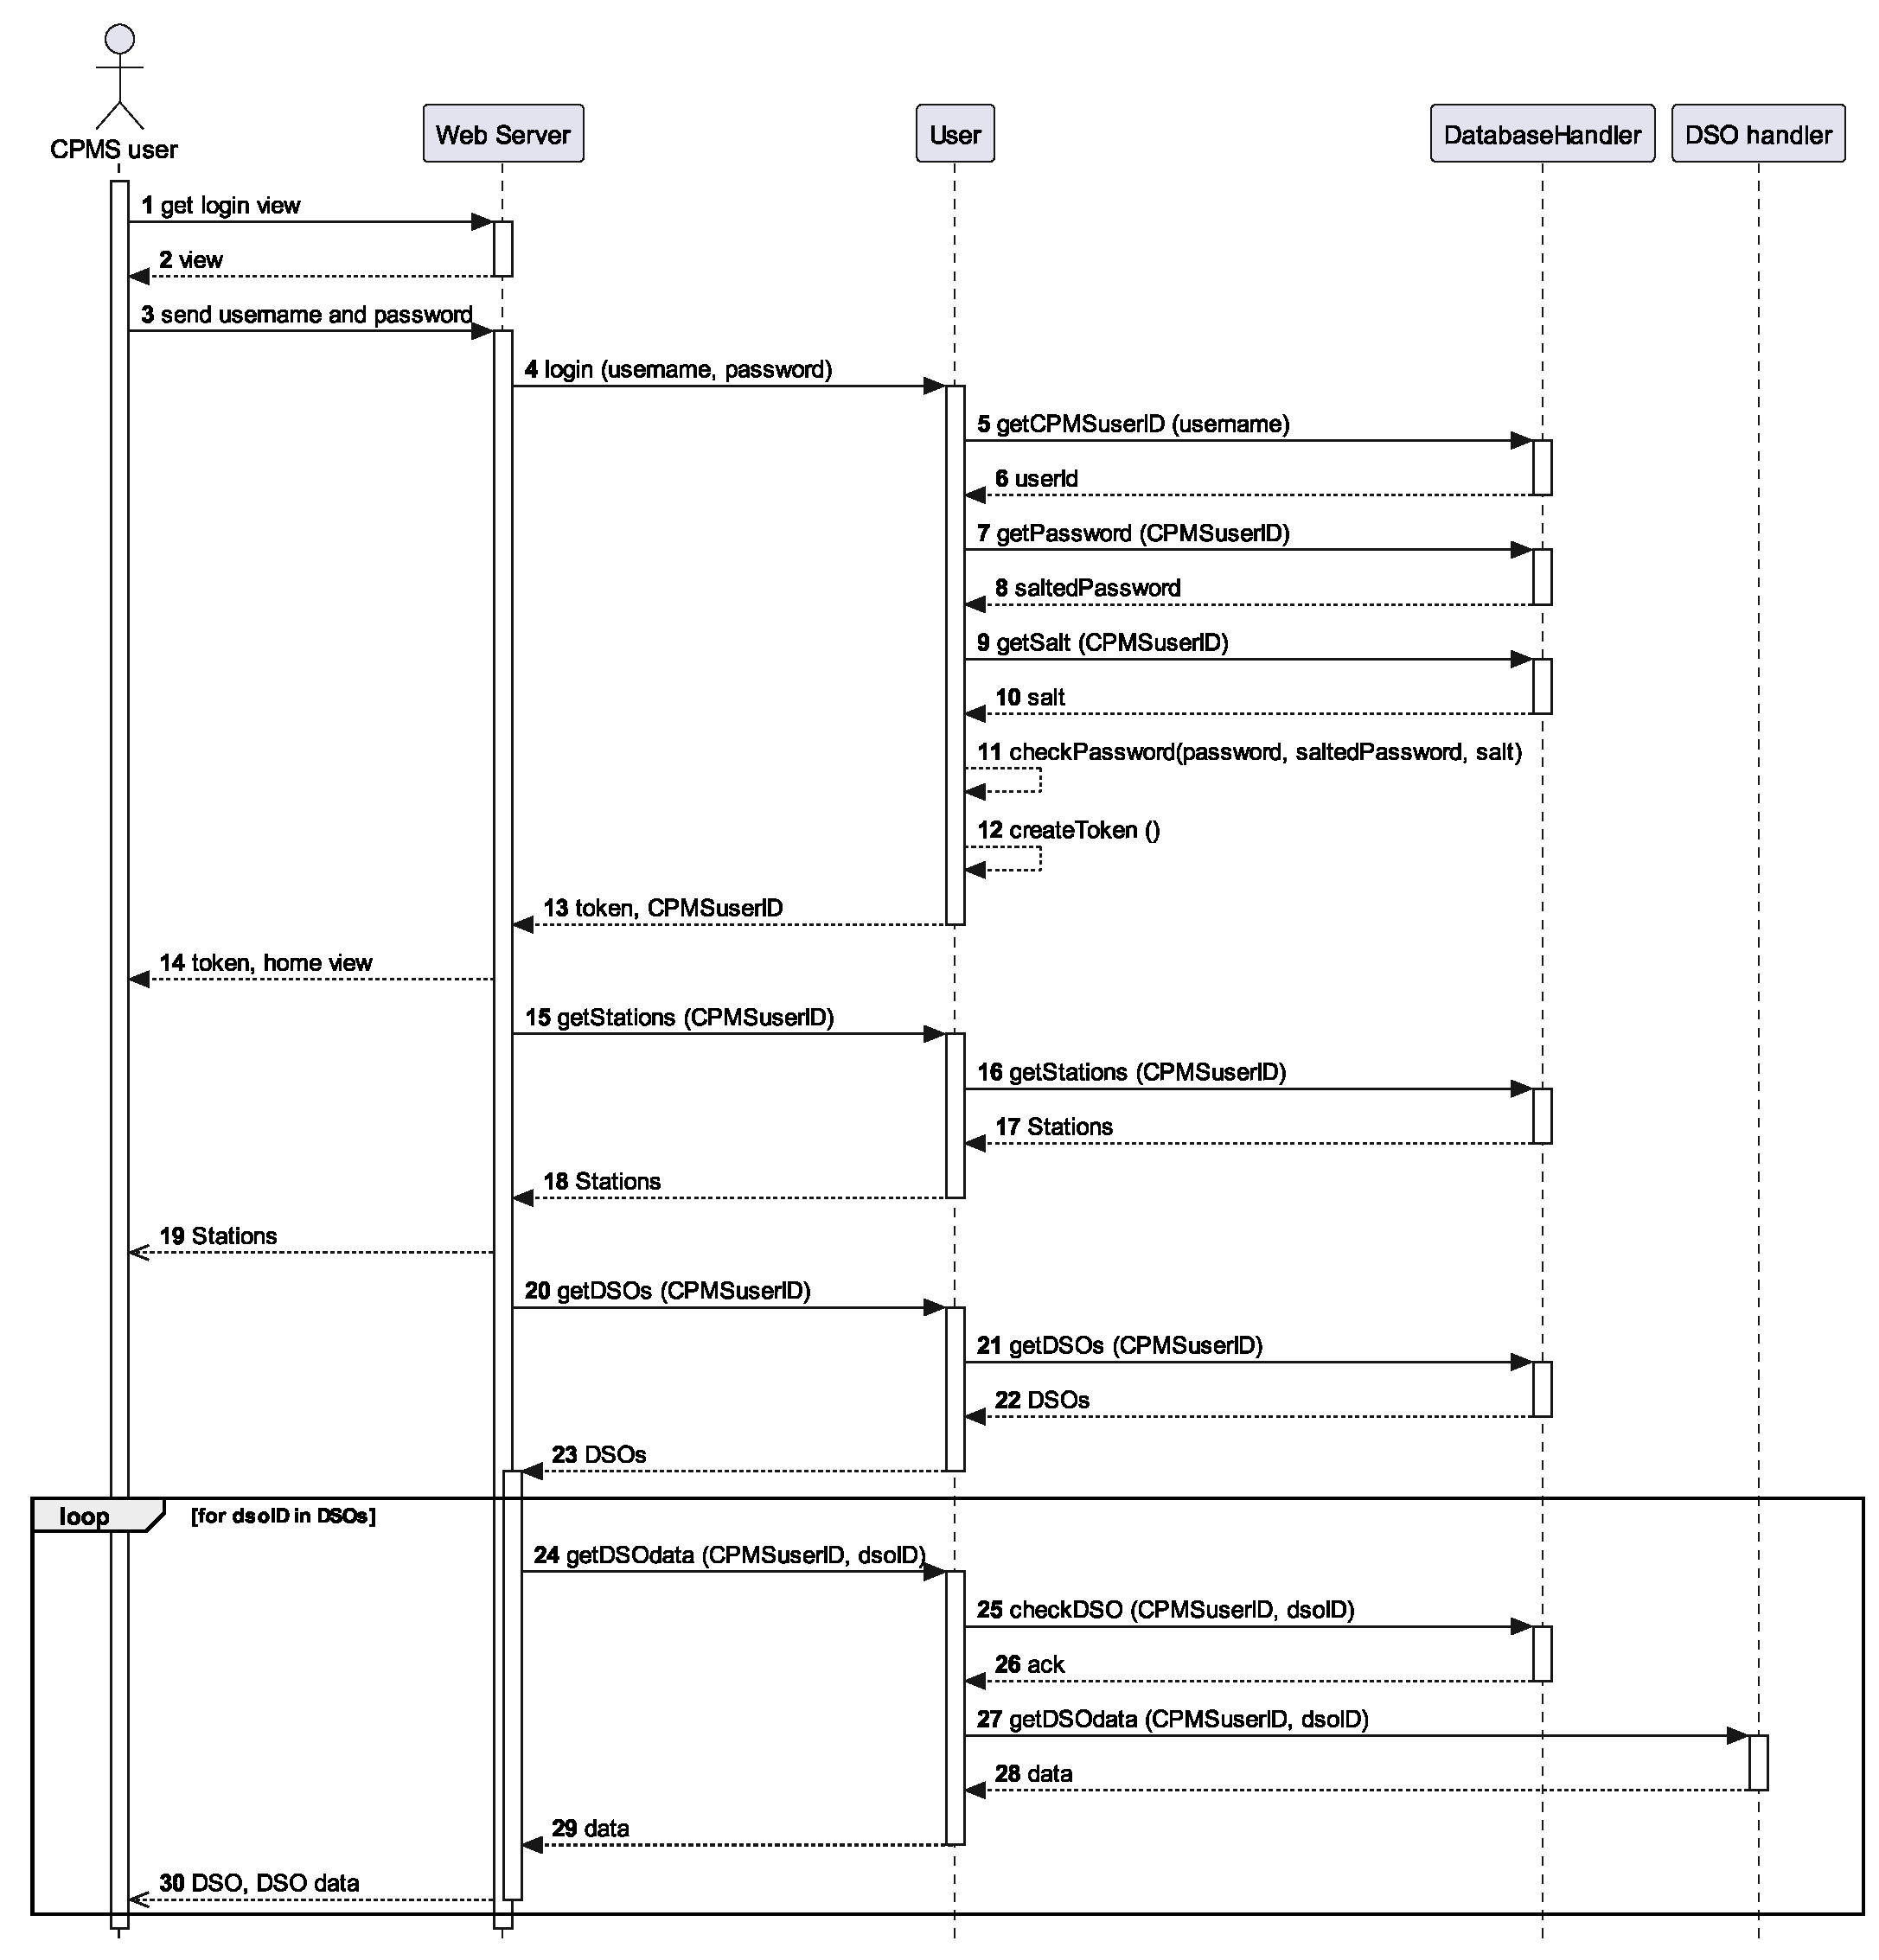
\includegraphics[width=\columnwidth]{./images/sequences/cpms/login}
    \caption{the user logs into the CPMS website.}
\end{figure}

\pagebreak

\paragraph{Monitoring a station} In the \doublequotes{Station} view users can monitor the situation inside stations. Until they leave the page, the \texttt{Web Server} will run an asynchronous periodical loop to fetch new information to send in JSON files. 

\begin{figure}[h!]
    \centering
    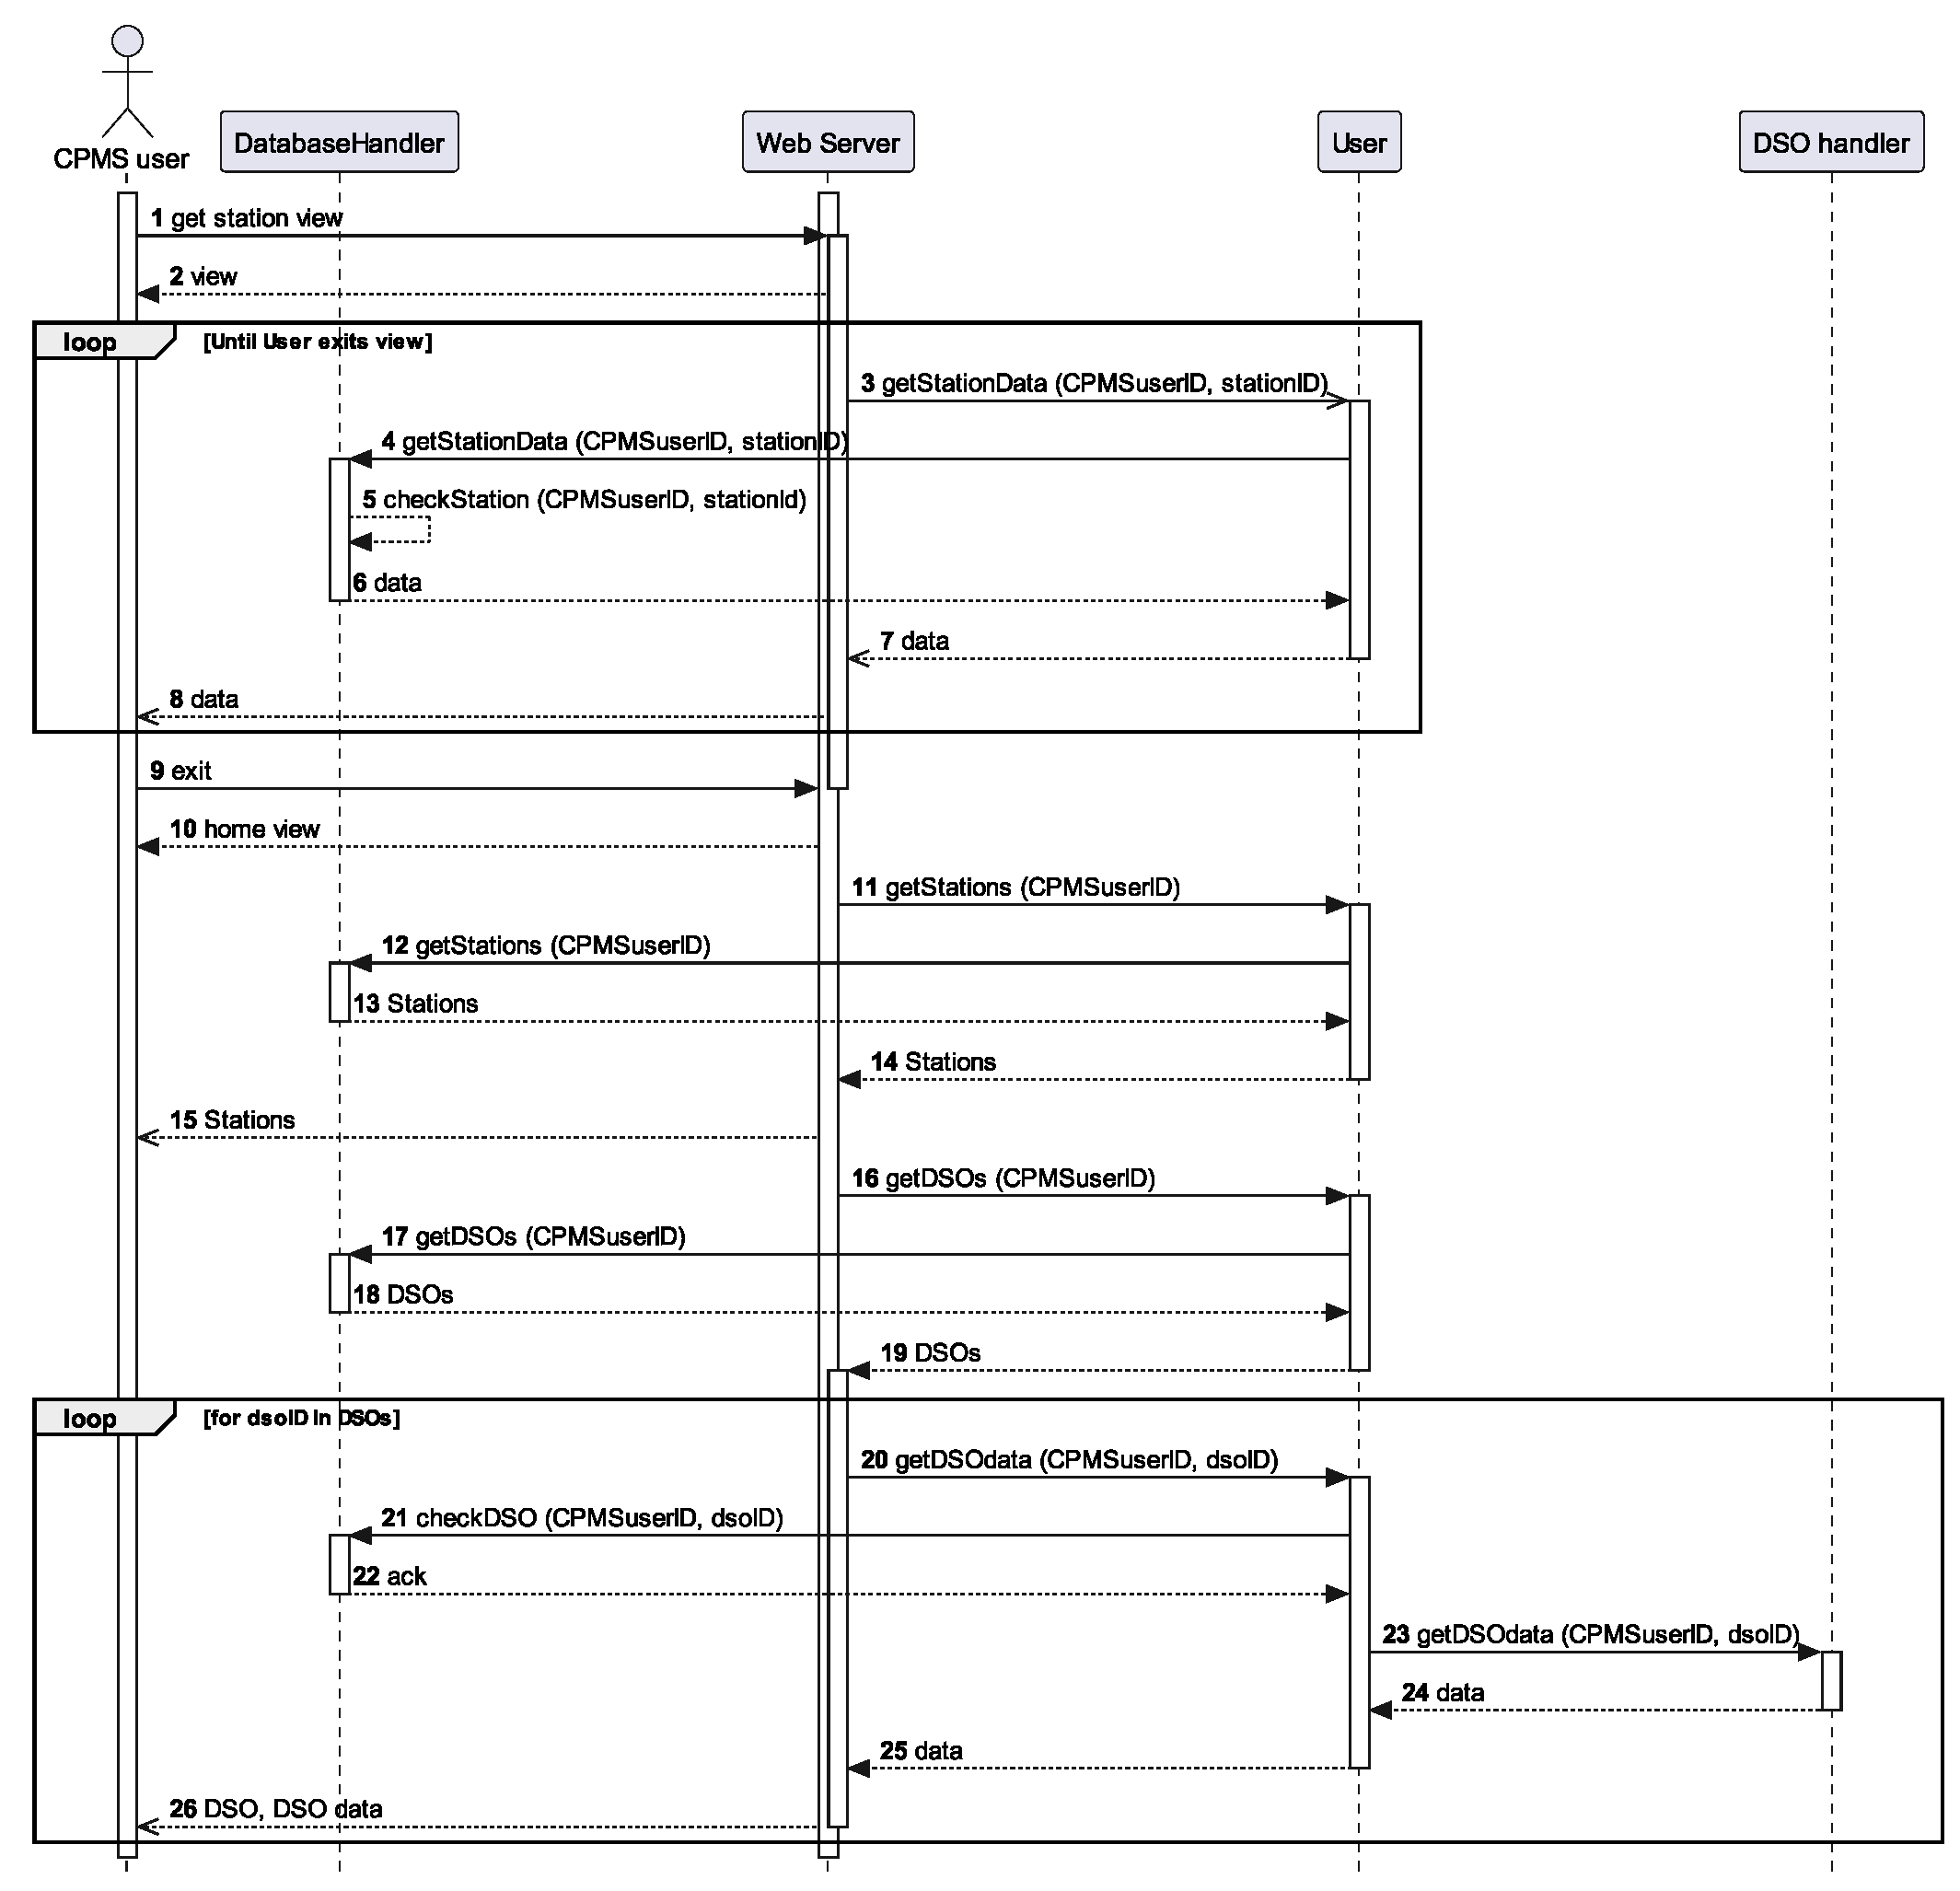
\includegraphics[width=\columnwidth]{./images/sequences/cpms/monitor}
    \caption{the user selects a station to view, then goes back to the home page.}
\end{figure}

\pagebreak

\paragraph{Activating automatic energy mix} From a \doublequotes{Station} view, the user selects \doublequotes{Automatic Mix choice}, then decides to log out. Since \doublequotes{automatic mix} is activated, the \texttt{ChargingStation} process enters a loop until this option is deactivated. In this loop, it periodically fetches information from sensors, decides what the best energy mix is, then waits some time.

\begin{figure}[h!]
    \centering
    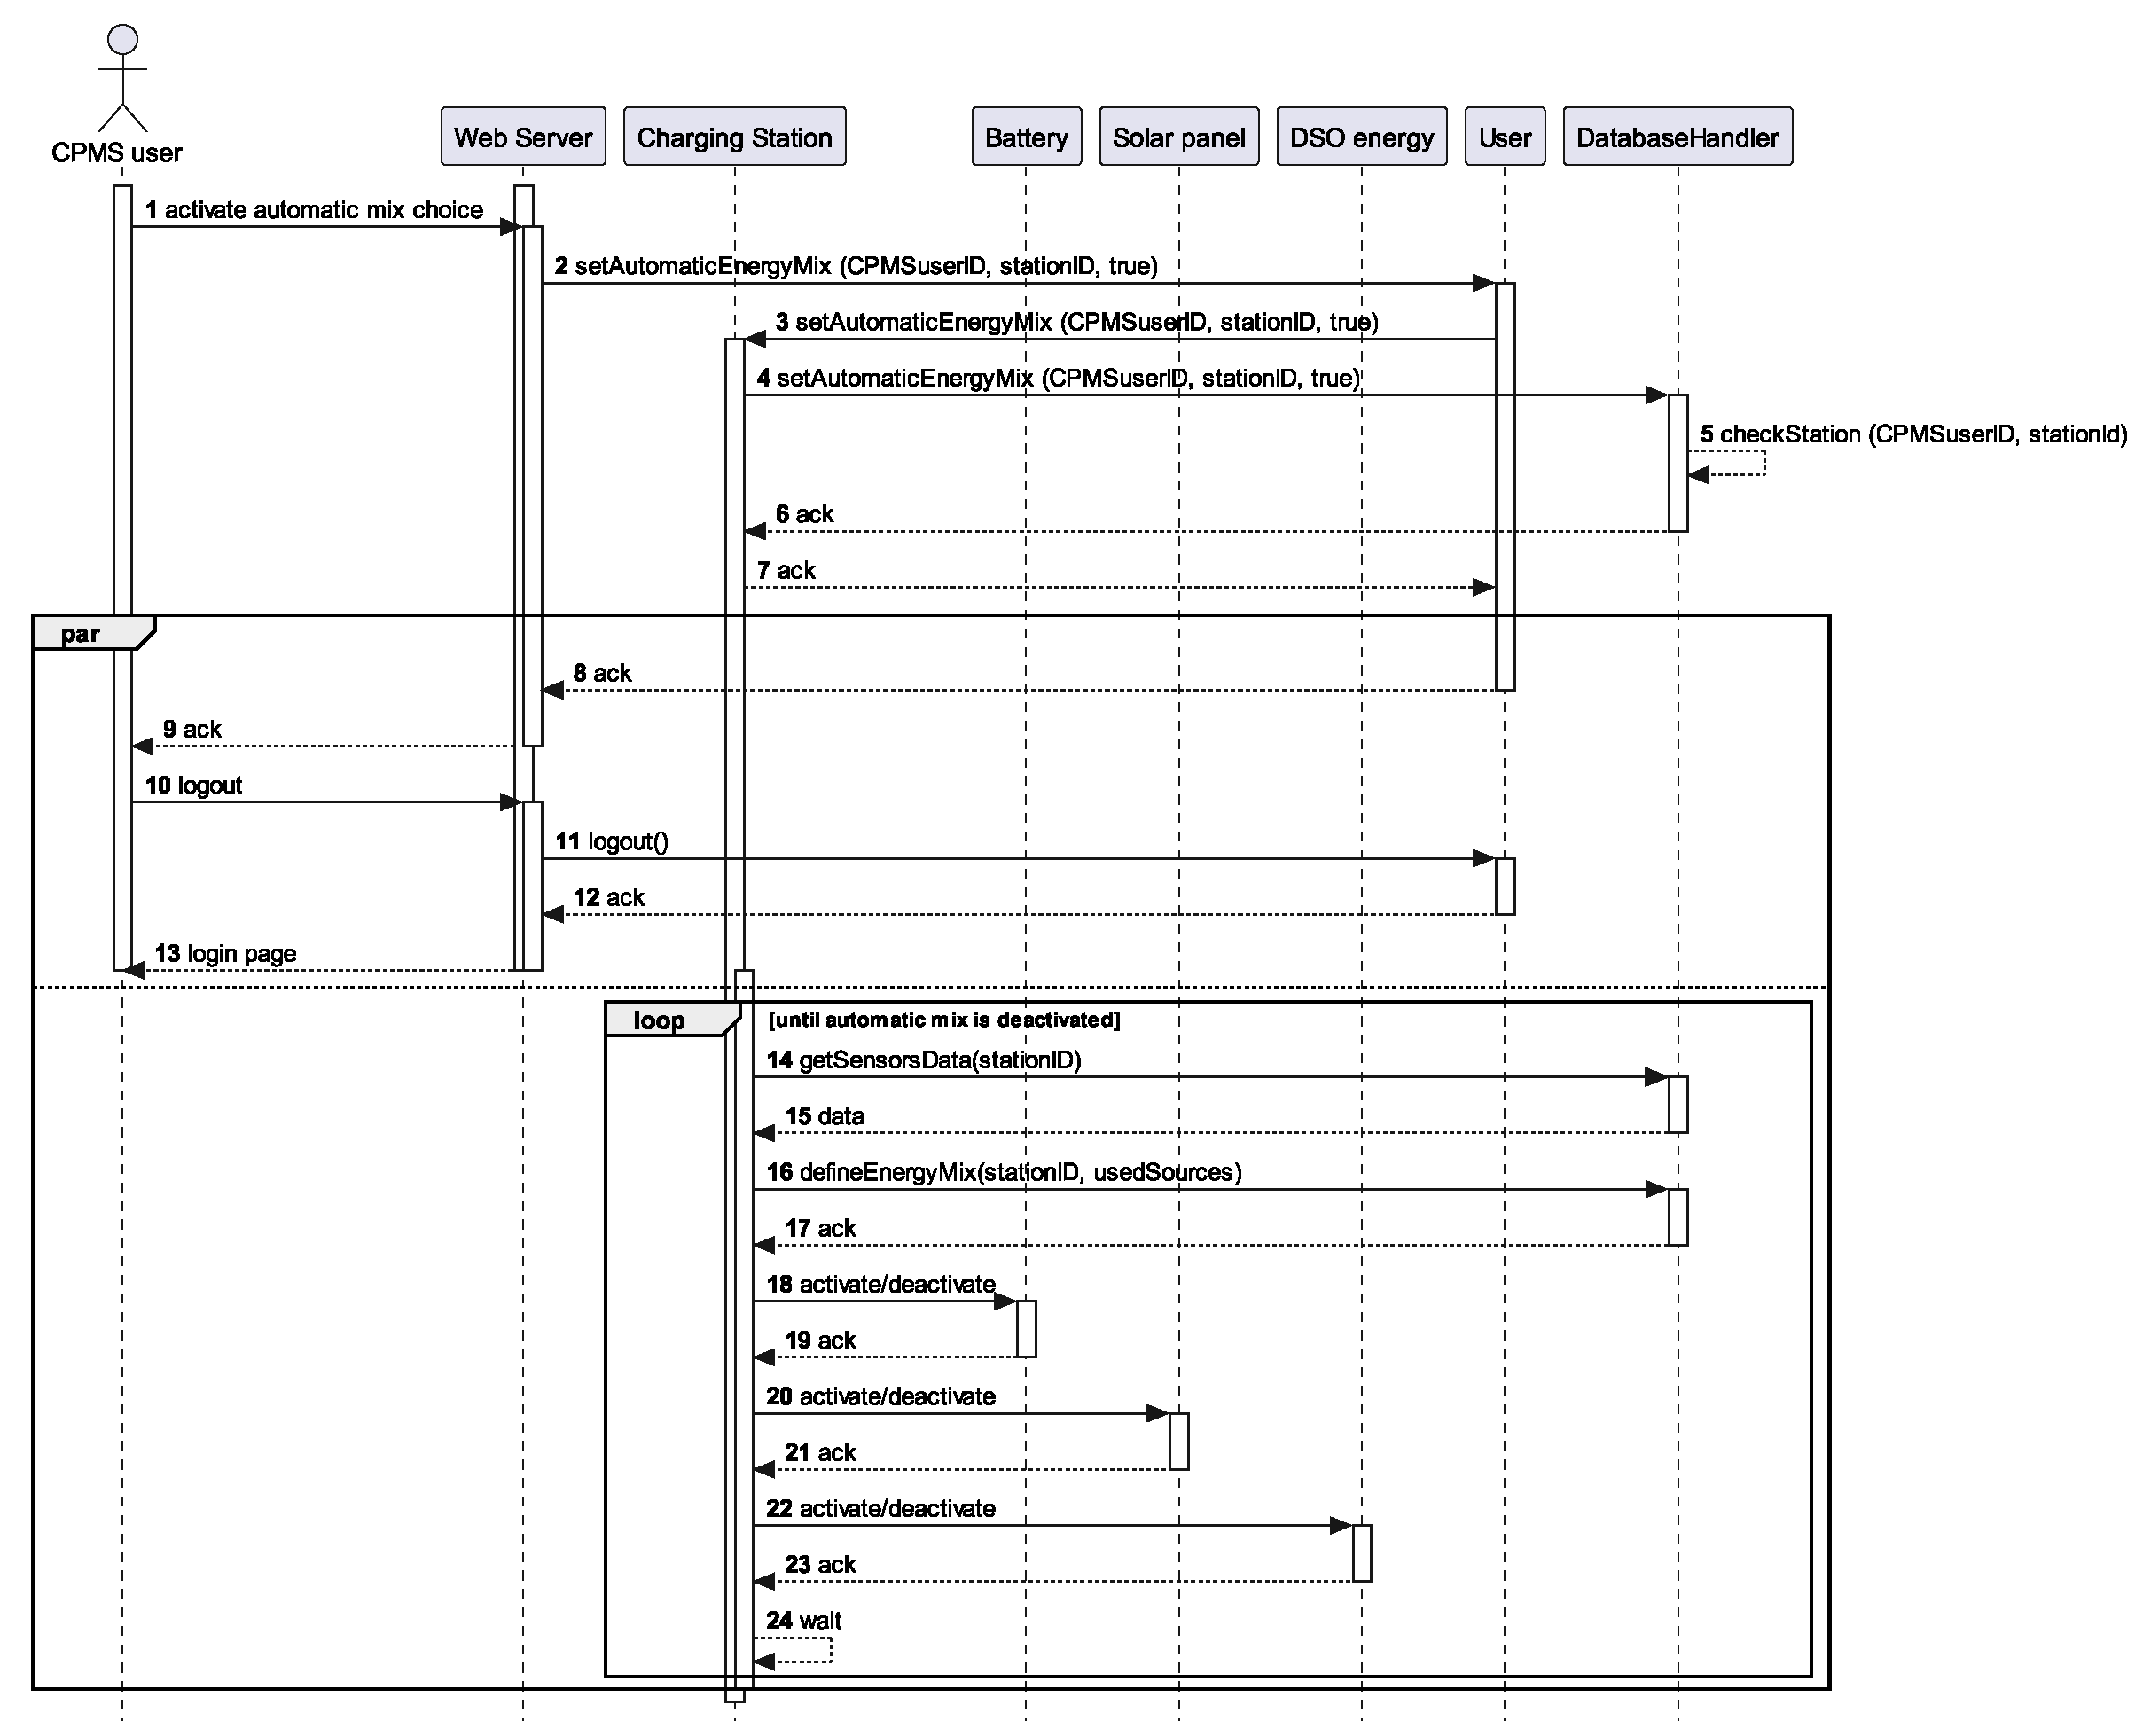
\includegraphics[width=\columnwidth]{./images/sequences/cpms/energyMix}
    \caption{the user activates automatic mix choice, then logs out of the website.}
\end{figure}

\pagebreak

\paragraph{DSO choice} From a \doublequotes{Station} view, the user selects \doublequotes{Automatic DSO choice}, then selects another DSO, ending the automatic choice. Since \doublequotes{automatic DSO choice} is activated, the \texttt{ChargingStation} process enters a loop until this option is deactivated. In this loop, it periodically fetches information from DSOs, decides what the best price is, selects that DSO, then waits some time.

\begin{figure}[h!]
    \centering
    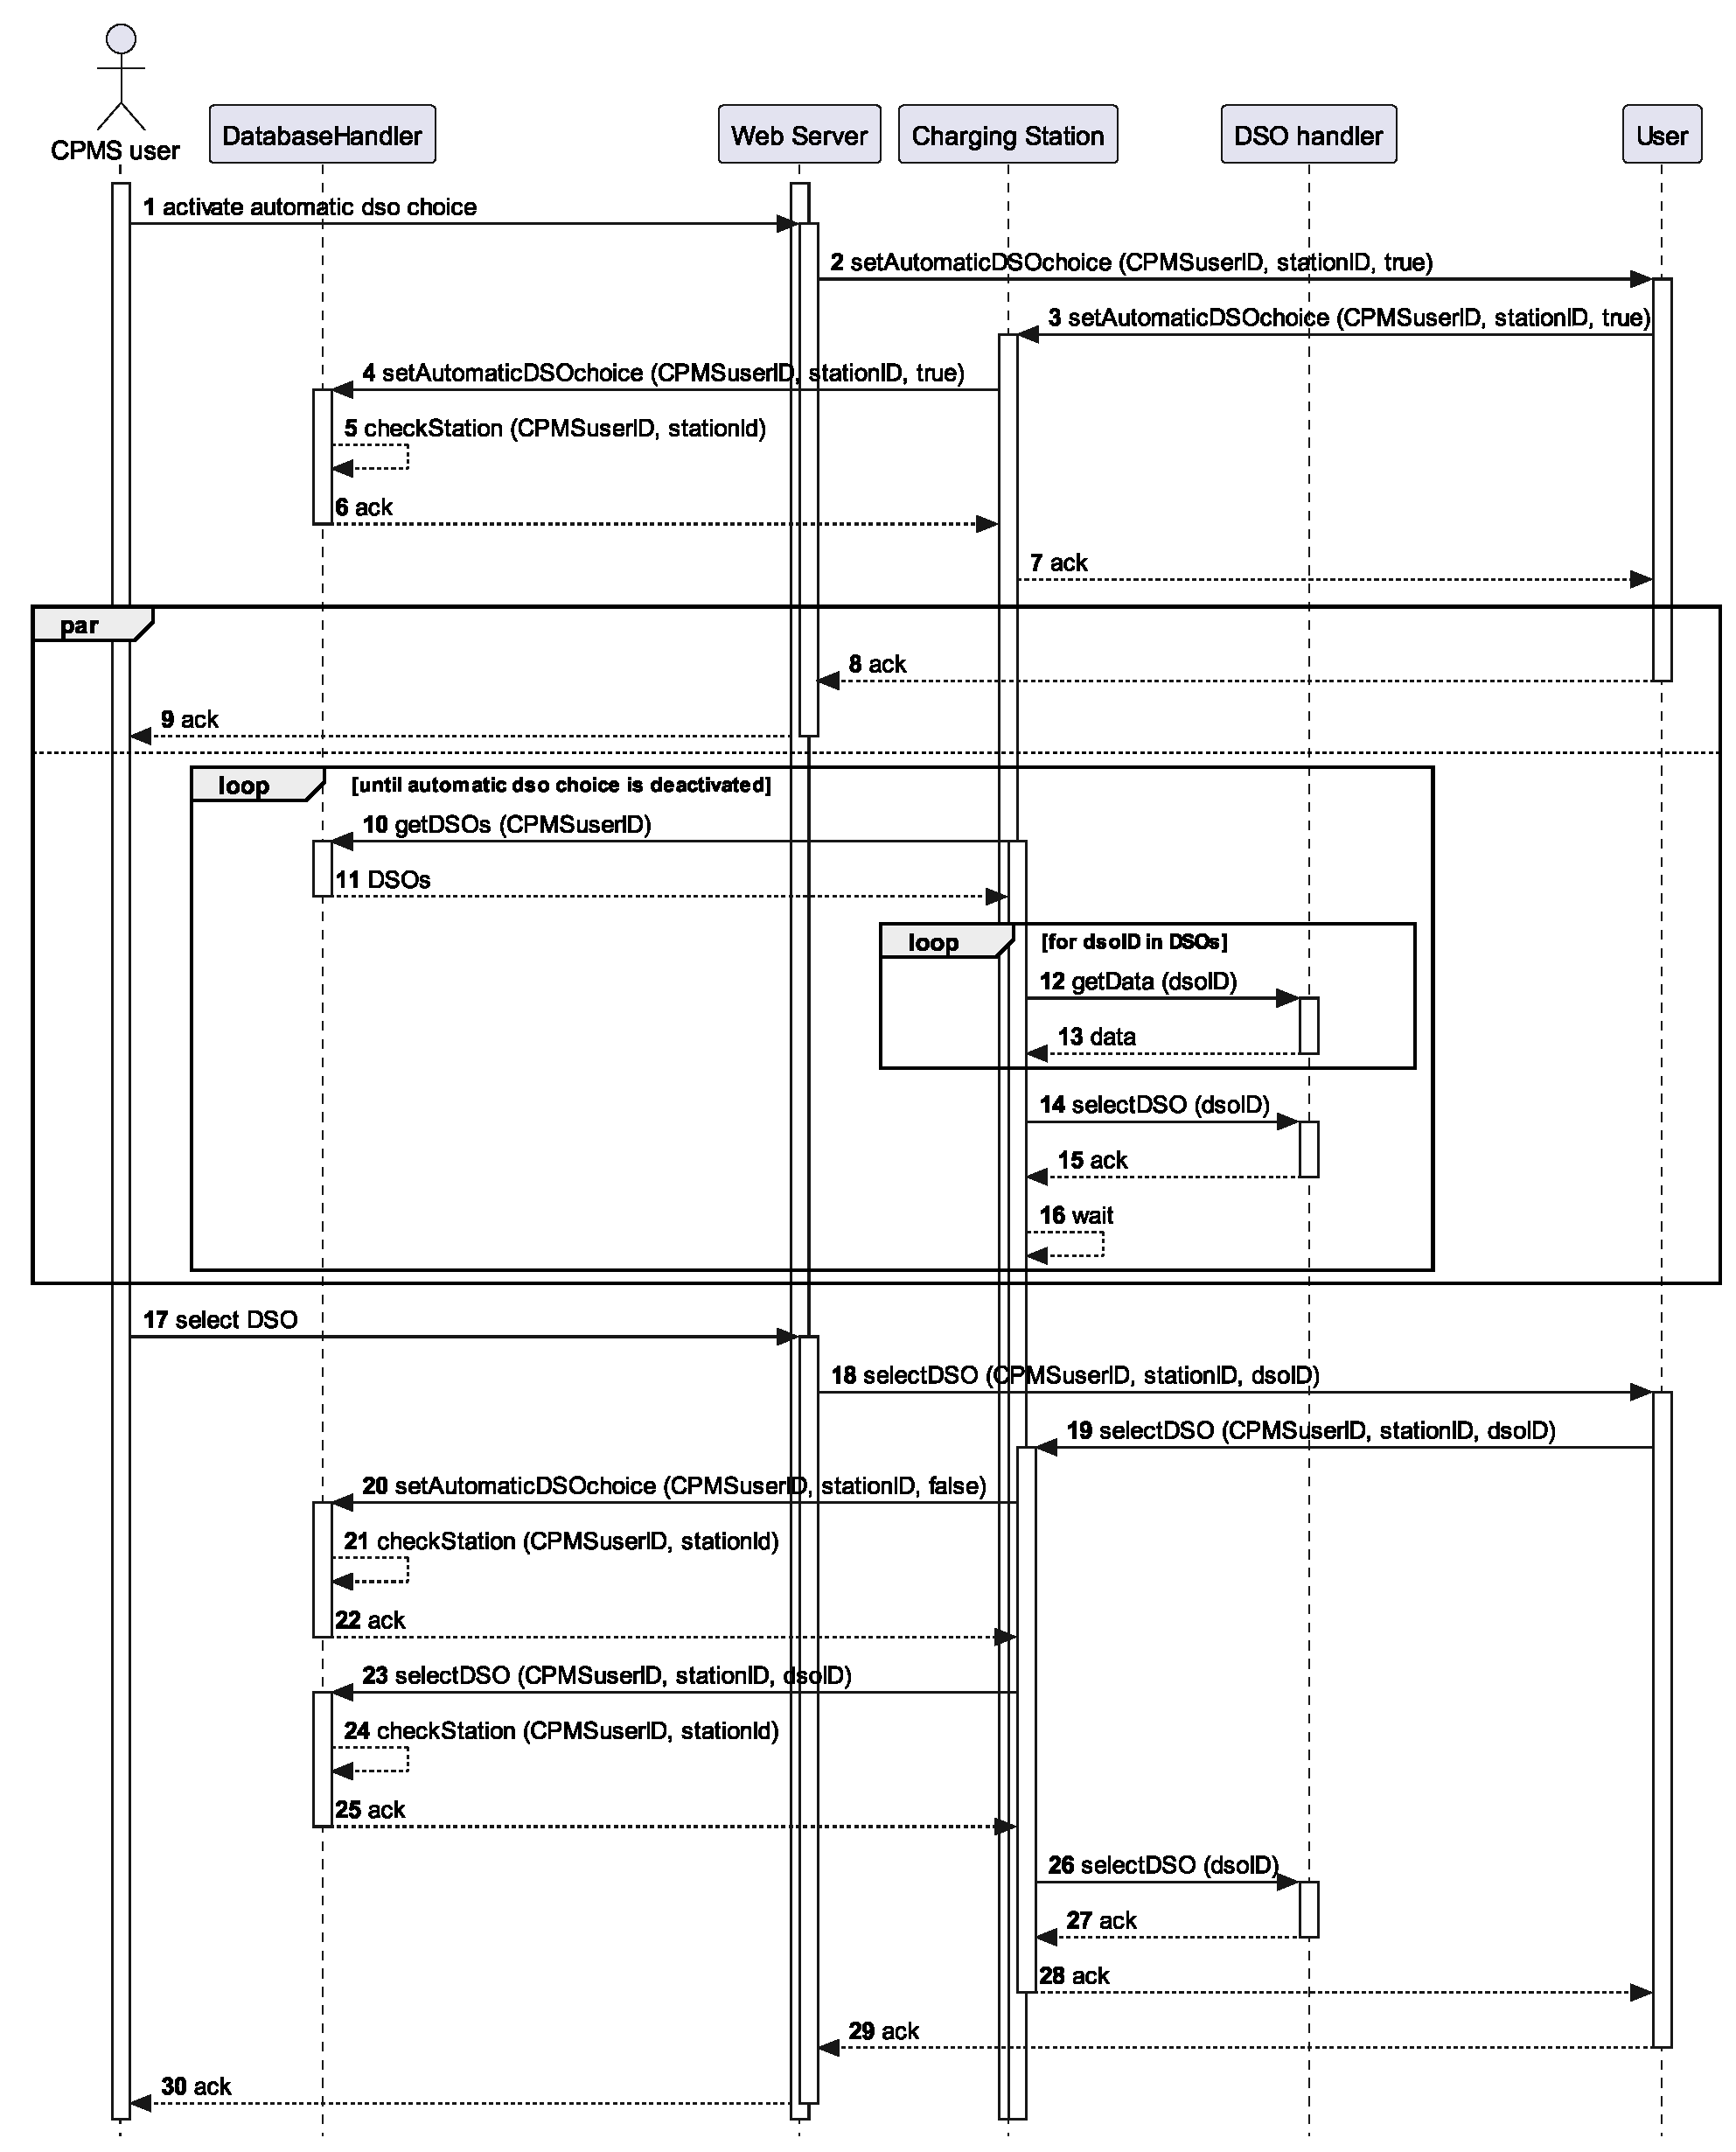
\includegraphics[width=\columnwidth]{./images/sequences/cpms/dso}
    \caption{the user activates automatic DSO choice, then deactivates it by selecting a specific DSO.}
\end{figure}

\pagebreak

\paragraph{Create a new special offer} The user enters the \doublequotes{Offer} view and creates a new special offer.

\begin{figure}[h!]
    \centering
    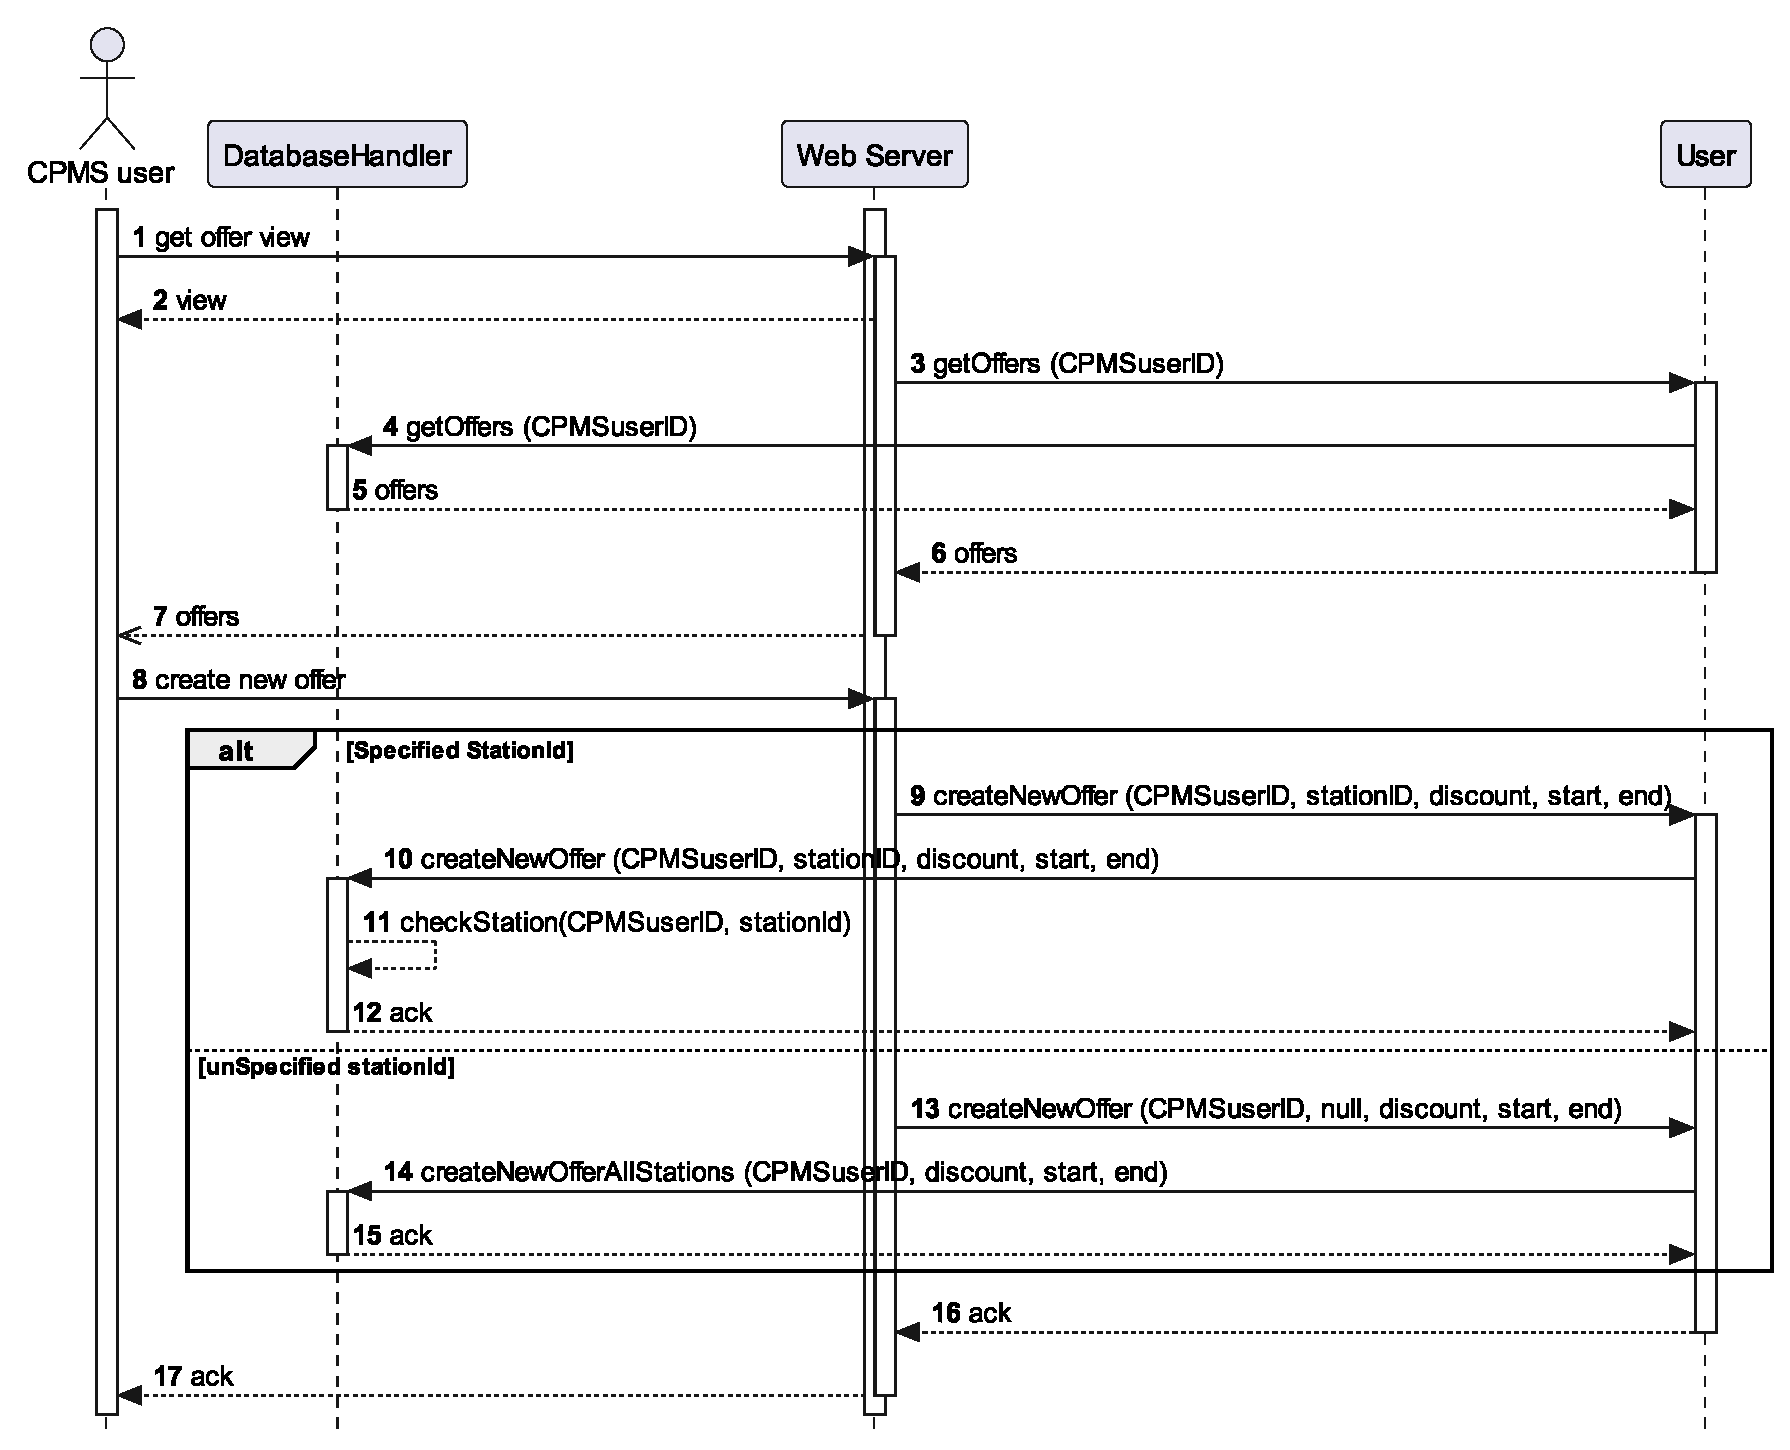
\includegraphics[width=\columnwidth]{./images/sequences/cpms/offers}
    \caption{the user creates a new special offer.}
\end{figure}

\paragraph{Other functions} The CPMS system allows for other actions to occur, but they are not depicted here because they are fairly basic, and their diagram can be better described with words. Every notification to the eMSP is sent through the \texttt{sendNotification (eMSP\_ID, eMSPuserID, message)} function of the \texttt{eMSPinterface}. eMSP users are allowed to pay the charge at the charging station, therefore \texttt{ChargingColumn} can access the \texttt{PaymentInterface} in order to use the function \texttt{payCharge (eMSPuserID, paymentData)}. eMSP add, delete, update and query bookings through the use of the various \doublequotes{Booking} functions of the \texttt{BookingInterface} and the \texttt{DatabaseInterface}. eMSPs are added to the database though the function \texttt{add\_eMSP (eMSP)} called by the eRoamingHandler.

\pagebreak

\section{Selected architectural styles and patterns}

Here are presented all the design patterns that have been chosen for building up the two systems, which are very similar in this aspect.

\subsection{Three-tier architecture}

Both the eMSP and the CPMS present a three-tier architecture. This is because it helps to divide the local functions of every component into three different \doublequotes{classes} (presentation, business and data) which have different duties. The presentation layer is in charge of directly answering the user's requests, activating the required components in the backend, and collecting the final answer. The data layer is in charge of keeping organized all the data of the system. Finally, the business is the logical core of the system, indeed it provides the needed answers to the frontend by indirectly analyzing the requests from the client and picking and processing the required data from the data layer.

\subsection{Microservice architecture}

Both the eMSP and the CPMS present a microservice architecture. This design decision has been taken because it allows the system to be more resilient, to be able to scale better (e.g. duplicating the bottleneck components) and it can also be developed, updated, and tested by different teams, allowing a faster startup.

\subsection{Containerized architecture}

Both the eMSP and the CPMS present a containerized business layer. For providing even stronger security and resilience to failures, all those components are containerized, which means that all run on a different \doublequotes{virtual} environment, without the knowledge of the whole system on which they are running. Thanks to the use of a Kubernetes service, it's possible to orchestrate multiple machines in order to proactively react to the traffic to the service and easily update components. This can be done thanks to the volatile nature of the containers, which can be brought up and down and updated in a really easy way.

\subsection{Database-centric architecture}

Both the eMSP and the CPMS present a database-centric architecture. This implies that every component relies on the database for obtaining data and processing information. In case of failures of components, they can be restarted without any loss since all the information is stored in the database, which, itself, is a replicated piece of software.

\subsection{RESTful architecture}

Both the eMSP and the CPMS present a RESTful architecture. This is especially true in the client-server relation since the client only asks the server for HTML, CSS and JavaScript files for correctly visualizing pages (which is not required in the case of the eMSP's mobile application) and then queries the server through standard HTTP requests for the required data, providing a JWT at every request for being recognized.

\subsection{Observer design pattern}

Components in the CPMS system can implement the observer pattern: \texttt{ChargingColumn} and \texttt{EnergySource} offer through their interfaces the \texttt{addObserver (observer)} function, \texttt{ChargingStation} can then add observers to them. These observers are used to prevent in-station batteries from passing a certain charge level or to send a notification when the user's car's charge ends.
